%==============================================================================
%  Explainable AI-Based Phishing Website Detection
%  A Human-Centred Machine Learning and SHAP-Based Framework
%  LaTeX source converted from the original Word report.
%
%  Compile with pdflatex (run twice for the table of contents / cross-refs):
%      pdflatex main.tex
%      pdflatex main.tex
%==============================================================================
\documentclass[11pt,a4paper]{article}

%------------------------------- Packages -------------------------------------
\usepackage[utf8]{inputenc}
\usepackage[T1]{fontenc}
\usepackage[a4paper,margin=1in]{geometry}
\usepackage{amsmath,amssymb}
\usepackage{graphicx}
\usepackage{booktabs}
\usepackage{longtable}
\usepackage{array}
\usepackage{tabularx}
\usepackage{ragged2e}
\usepackage{caption}
\usepackage{float}
\usepackage{enumitem}
\usepackage{xcolor}
\usepackage[hidelinks,colorlinks=true,linkcolor=black,citecolor=blue,urlcolor=blue]{hyperref}

%------------------------------- Settings -------------------------------------
\graphicspath{{figures/}}
\captionsetup[figure]{font=small,labelfont=bf,justification=justified}
\captionsetup[table]{font=small,labelfont=bf,justification=justified}
\setlength{\parskip}{0.5em}
\setlength{\parindent}{0pt}
\renewcommand{\arraystretch}{1.25}

% Convenience column types for tabularx (auto-wrapping, left/justified)
\newcolumntype{L}{>{\RaggedRight\arraybackslash}X}
\newcommand{\fig}[2]{%
  \begin{figure}[H]\centering
  \includegraphics[width=#2\linewidth]{#1}\end{figure}}

%==============================================================================
\begin{document}

%---------------------------- TITLE PAGE --------------------------------------
\begin{titlepage}
\centering
\vspace*{1.5cm}

{\large\textbf{University of Management and Technology}}\\[0.3cm]
{\normalsize School of Systems and Technology}\\[2.5cm]

{\Huge\textbf{Explainable AI-Based}}\\[0.4cm]
{\Huge\textbf{Phishing Website Detection}}\\[1.0cm]

{\large\itshape A Human-Centred Machine Learning and SHAP-Based Framework\\
for Non-Technical Users}\\[2.0cm]

\renewcommand{\arraystretch}{1.4}
\begin{tabular}{>{\bfseries}p{4.5cm} p{7.5cm}}
\toprule
Student name      & Ghulam Mustafa \\
Student ID        & F2023266976 \\
Degree programme  & BS Computer Science \\
Course / module   & Human--Computer Interaction \\
Supervisor        & Ms. Iqra Khalil \\
Institution       & University of Management and Technology \\
Submission date   & June 2026 \\
\bottomrule
\end{tabular}

\vfill
\end{titlepage}

%---------------------------- FRONT MATTER ------------------------------------
\pagenumbering{roman}

\tableofcontents
\clearpage

\listoffigures
\clearpage

\listoftables
\clearpage

%---------------------------- RESEARCH OVERVIEW -------------------------------
\section*{Research Overview}
\addcontentsline{toc}{section}{Research Overview}

\renewcommand{\arraystretch}{1.3}
\begin{tabularx}{\textwidth}{>{\bfseries}p{3.6cm} L}
\toprule
Field & Details \\
\midrule
Research area & Machine learning, explainable AI, cybersecurity, human--computer interaction \\
Dataset & Web Page Phishing Detection (dataset\_B\_05\_2020.csv), 11{,}430 instances, 87 features \\
Models evaluated & Logistic Regression, Decision Tree, Random Forest, Extra Trees, Gradient Boosting, XGBoost \\
Best model & XGBoost --- accuracy 0.96632, F1-score 0.96648, ROC-AUC 0.99443 \\
Explainability & Global feature importance and SHAP (global and local) explanations \\
Interface contribution & Human-centred warning \textbf{mock-up} translating model output into plain language \\
HCI evaluation & An 8-item Likert scale with a response workbook. The response values listed here are synthetic demonstration data to help illustrate the operation of the workbook and do not represent empirical data on usability or trust. \\
\bottomrule
\end{tabularx}

%---------------------------- ABSTRACT ----------------------------------------
\section*{Abstract}
\addcontentsline{toc}{section}{Abstract}

Phishing websites continue to be a dangerous cyber security threat as they mimic
trusted websites to get credentials, financial information and other personal data
from users. While phishing patterns can be identified with a high degree of accuracy
using machine learning, a lot of phishing classifiers are black-box tools and provide
little information for the user, who may dismiss or be skeptical of the warning if it is
not understandable. This study develops a human-centred explainable-AI framework for
phishing website detection using the Web Page Phishing Detection dataset, which contains
11{,}430 balanced instances (5{,}715 legitimate and 5{,}715 phishing) described by 87
numeric features derived from the URL, page content and external-reputation services.
Six supervised models were compared: Logistic Regression, Decision Tree, Random Forest,
Extra Trees, Gradient Boosting and XGBoost. Models were trained on an 80:20 stratified
split and assessed with accuracy, precision, recall, F1-score and ROC-AUC, supported by
five-fold stratified cross-validation. XGBoost achieved the strongest overall performance,
with a test-set accuracy of 0.96632, precision of 0.96187, recall of 0.97113, F1-score of
0.96648 and ROC-AUC of 0.99443, and a cross-validated mean F1-score of 0.96906
(SD $=$ 0.00202). Global feature importance and SHAP analysis identified
external-reputation signals (notably Google indexing and PageRank) and URL/page-structure
features as the most influential, and these were translated into plain-language warnings
within a proposed interface mock-up. An eight-item Likert evaluation instrument and a
structured response workbook were designed to support future usability testing; the
response values reported here are synthetic demonstration data and do not establish
usability, trust or user acceptance. The paper demonstrates that correct phishing
detection must be accompanied with explanation and user-centred warning design to help
users make safer decisions in terms of browsing.

\vspace{0.5em}
\noindent\textbf{Keywords:} cybersecurity; explainable AI; human--computer interaction;
machine learning; phishing detection; SHAP; XGBoost.

\begin{figure}[H]\centering
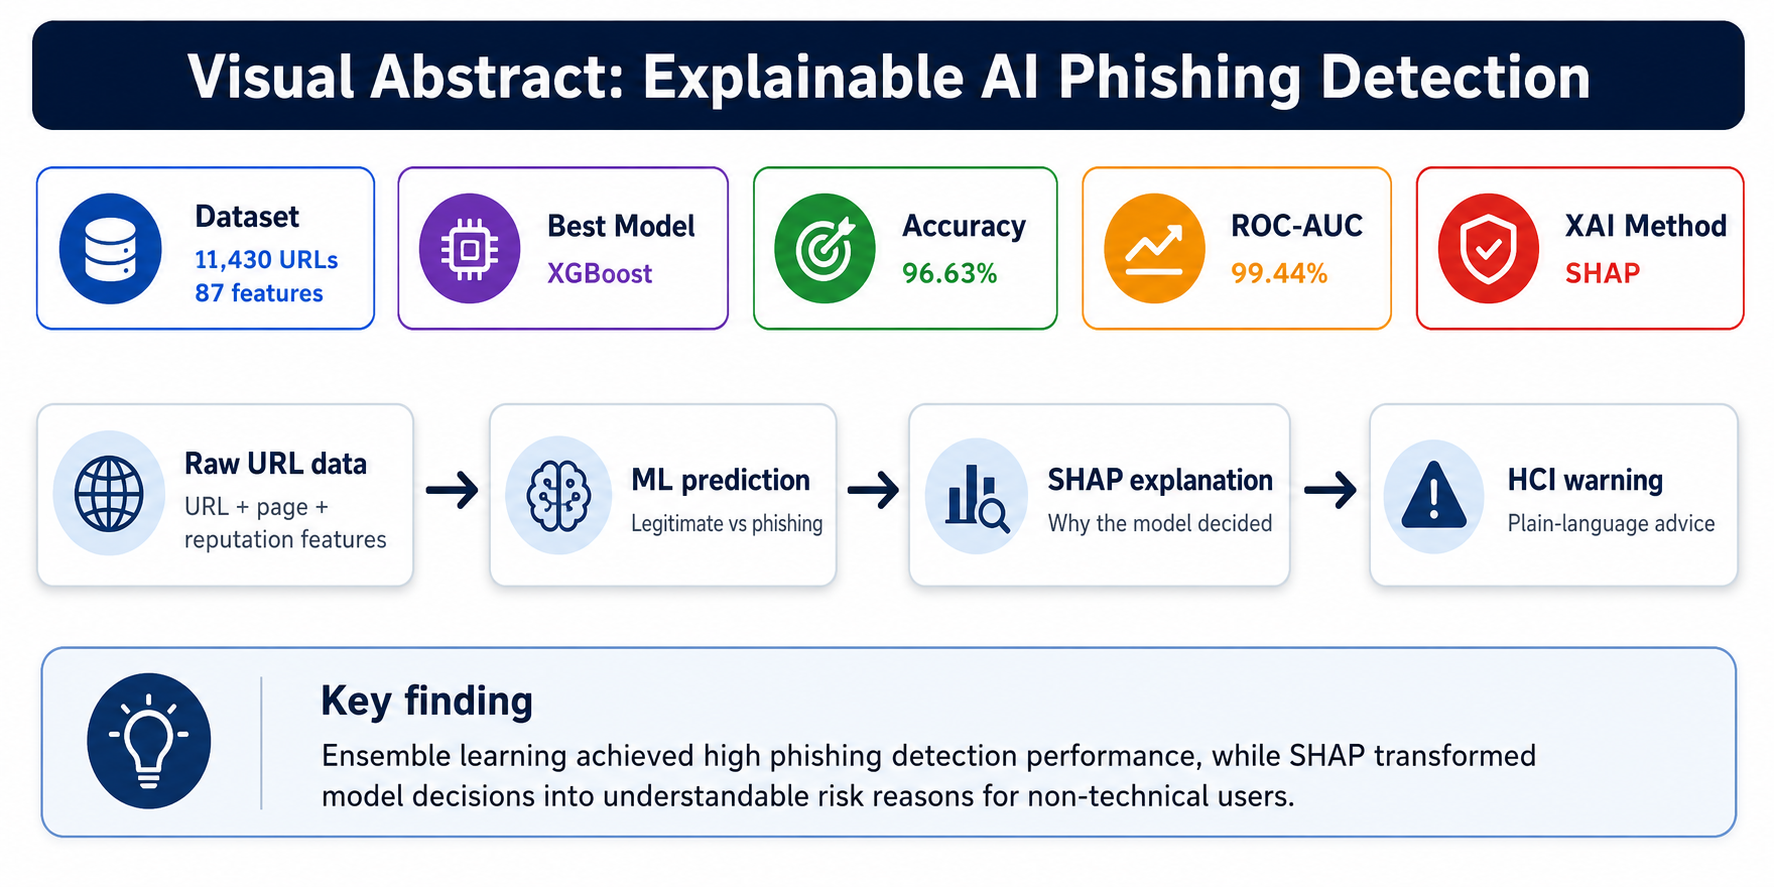
\includegraphics[width=0.95\linewidth]{figure01.png}
\caption{Visual abstract: the dataset, ensemble model, best result and SHAP-based
explanation that make up the study at a glance. Source: Authors' design.}
\label{fig:visual-abstract}
\end{figure}

\clearpage
\pagenumbering{arabic}

%==============================================================================
%  Body of the report: Sections 1-11, References, Appendix A
%==============================================================================

%================================ 1. INTRODUCTION =============================
\section{Introduction}

Phishing is an ongoing cybersecurity issue where malicious sites mimic genuine sites
and deceive users into divulging sensitive data. These sites are usually not vulnerable
technically but through interface familiarity, feelings of urgency, social-engineering
triggers and visual similarity. As online banking, cloud services, e-commerce and
academic services continue to grow, it has become increasingly easy to create a
convincing phishing page, and increasingly difficult for the average internet user to
identify one.

Machine learning can detect phishing patterns across the structure of a URL, the content
of a page and external-reputation signals. But if the user does not know or trust the
warning from a highly accurate classifier, then the classifier will not be effective. An
alert that a non-technical user receives may be ignored, not trusted, or misinterpreted,
leading them to believe that they have no concern about the alert. A number of classifiers,
however, are black box in nature, thus restricting their use as ubiquitous decision-support
tools. This study fills this gap by using predictive modelling with explainable AI (XAI)
and Human--Computer Interaction (HCI) to communicate, in plain language, why a page is
deemed risky and what the user should do, while also predicting whether the website is a
phishing site or not.

We need to make a distinction between the four contributions of this work. The first one
is predictive model development, where six supervised models are trained and compared. The
second is explainability analysis: global feature importance and SHAP are calculated for
the best model. The third one is the user-centred warning mock-up, which translates the
model outputs into user-centred warnings. The fourth is the evaluation tool: an eight-item
Likert questionnaire and a structured response workbook are prepared for future user
testing. No browser extension or live detector was implemented or tested; this is only a
design prototype of the interface.

The rest of this paper is organised as follows. Section~2 summarises the related work on
phishing detection, explainable AI and warning design. The research aim, objectives and
questions are then stated in Section~3. The research method is described in Section~4.
Experimental results are given in Section~5. The explainability analysis and human-centred
interface are presented in Section~6. The HCI evaluation instrument is shown in Section~7.
The discussion, ethical considerations, limitations and future work, and the conclusion are
provided in Sections~8--11.

\begin{table}[H]
\caption{Research problem mapping.}
\label{tab:problem-mapping}
\centering\footnotesize
\begin{tabularx}{\textwidth}{L L L}
\toprule
\textbf{Current problem} & \textbf{Research gap} & \textbf{Proposed response} \\
\midrule
Phishing websites imitate trusted services and deceive users. &
Detection systems often prioritise model accuracy over user understanding. &
A machine-learning detector paired with user-facing explanations. \\
Black-box models provide limited explanation. &
Non-technical users may not trust or follow warnings. &
SHAP and plain-language explanations of model output. \\
Security warnings can be unclear or overly technical. &
HCI evaluation is frequently absent from phishing-detection studies. &
An HCI evaluation instrument and a structured response workbook. \\
\bottomrule
\end{tabularx}
\end{table}

\begin{figure}[H]\centering
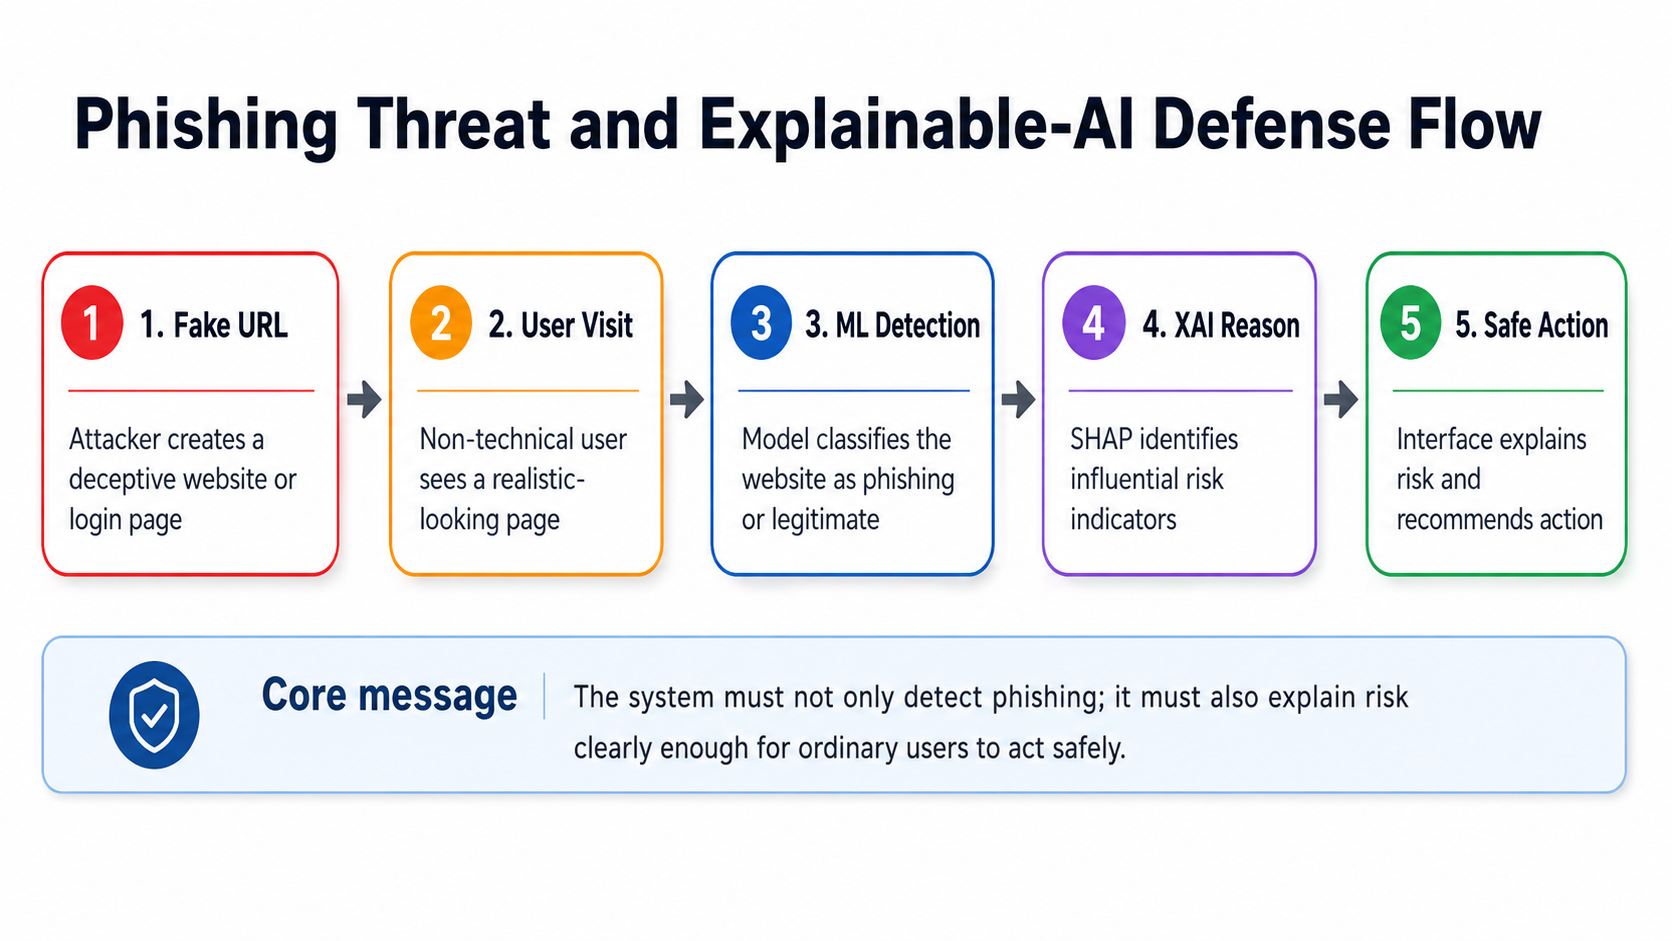
\includegraphics[width=0.92\linewidth]{figure02.png}
\caption{Phishing threat and explainable-AI defence flow, from a deceptive URL through
model detection and SHAP-based reasoning to a clear user warning. Source: Authors' design.}
\label{fig:threat-flow}
\end{figure}

%================================ 2. LITERATURE REVIEW ========================
\section{Literature Review}

\subsection{Phishing Website Detection Approaches}

There are a number of complementary strategies that have been developed to detect phishing.
Blacklists are lists of known malicious URLs that are fast and accurate, but cannot
recognise new domains due to the short lifetimes of many phishing sites. Heuristic and
rule-based systems represent knowledge by a set of hand-crafted rules; they are easily
interpretable but brittle and need frequent manual changes. URL-based detection checks the
length of the URL, unusual characters, host properties and IP-address use. In content-based
detection, forms, hyperlinks, embedded scripts and even the login fields of the page are
studied. Reputation-based detection relies on metrics such as web traffic, domain age and
search-engine indexing. Visual-similarity methods compare the photo-realistic representation
of a candidate page to that of authentic brands. More recent work uses machine-learning and
deep-learning approaches, which learn patterns directly from large feature sets, with a
better ability to generalise to new, unseen pages than static rules or lists~\cite{ref1,ref2}.

\subsection{Machine Learning for Phishing Detection}

Supervised classifiers have been widely applied to the problem of phishing detection on
structured-feature sets. Logistic Regression offers a linear baseline that is easily
interpreted but is unable to account for complex non-linear interactions. A single Decision
Tree is easy to understand but can over-fit. Ensemble methods exist to overcome these
weaknesses: Random Forest averages many decorrelated trees, and Extra Trees brings more
randomisation for robustness on tabular data. Gradient Boosting adds trees one after another
to minimise previous errors, while neural-network methods also work well when there is a lot
of raw data (character-level URLs, page screenshots) but are not as competitive as
gradient-boosted trees on moderate-sized tabular feature sets, and are less interpretable.
The features in phishing are heterogeneous, the relationships between different features are
non-linear, and axis-aligned splits handle them well; hence the use of tree-based ensembles
works well here~\cite{ref2,ref5}.

\subsection{Explainable AI in Cybersecurity}

An accurate but opaque model offers little support for human security decisions. Explainable
AI enables us to differentiate global explanations, which explain overall model behaviour,
from local explanations, which explain the reasoning behind a given prediction.
Feature-importance scores rank the inputs based on their overall contribution. SHAP gives
each feature its contribution to a particular prediction with the help of Shapley values from
cooperative game theory, giving a consistent and locally accurate explanation of why a page
was classified as phishing or legitimate~\cite{ref3}. LIME, on the other hand, provides a
complementary approach by simplifying the model in the neighbourhood of a specific instance to
approximate it~\cite{ref4}. The advantages of SHAP are that it is based on a sound theoretical
framework, provides additive local explanations and offers informative summarising
visualisations; its disadvantages are that it is computationally expensive and that feature
attributions can be mistaken for causal effects. For security decision support, explanations
need to be faithful to the model but also easy enough for a non-expert to follow and act upon.

\subsection{Human--Computer Interaction and Warning Design}

HCI research reveals that the effectiveness of a security warning relies not only on the
accuracy of the detector underpinning it, but also on the design of the warning itself.
Warnings should be understandable, include good risk communication and be
actionable~\cite{ref6,ref7}. If warnings are repeated or of poor quality, they can lead to
warning fatigue and habituation, whereby the user no longer pays attention. Good designs avoid
jargon and use colour and visual hierarchy to emphasise severity (in a way that is
understandable to people with colour-vision defects) and clearly define what the user should
do next. A key objective is proper trust calibration: if the system is likely to be correct,
the user should rely on it, and if it is not, the user should be careful---but not take it for
granted. Research on the reasons for phishing's success focuses on the need for non-technical
users to be told about the risks they can see, rather than the technical details~\cite{ref8}.

\subsection{Research Gap}

The phishing-detection literature tends to focus on predictive performance and neglect
factors of human understanding, explanation quality, warning usability, trust calibration and
decision support. Few studies have combined the three fields into a single end-to-end pipeline
for the user. This study tackles that issue by integrating a well-performing classifier with
SHAP-based explanations and warning design based on human factors, and by creating a
structured instrument that can be used for empirical evaluation of usability, explanation
clarity, trust and decision support in the future.

%================================ 3. AIM, OBJECTIVES =========================
\section{Research Aim, Objectives and Questions}

The aim of this study is to design and assess an explainable-AI framework for phishing
website detection that accurately classifies websites and presents understandable, actionable
warnings to non-technical users.

\begin{table}[H]
\caption{Research aim, objectives and research questions.}
\label{tab:objectives}
\centering\footnotesize
\begin{tabularx}{\textwidth}{L L}
\toprule
\textbf{Objective} & \textbf{Related research question} \\
\midrule
O1. Pre-process and analyse the Web Page Phishing Detection dataset. &
RQ1. What are the characteristics and class balance of the dataset? \\
O2. Compare six supervised models for phishing classification. &
RQ2. Which model achieves the strongest overall performance? \\
O3. Identify the most influential URL, page-content and external-service features. &
RQ3. Which features contribute most to phishing predictions? \\
O4. Apply SHAP to explain global and individual predictions. &
RQ4. How can explainable AI improve the transparency of the detector? \\
O5. Design a plain-language warning interface mock-up for non-technical users. &
RQ5. How can model output be presented to non-technical users? \\
O6. Develop an HCI evaluation instrument for usability, clarity, trust and decision support. &
RQ6. How can usability, explanation clarity, trust and decision support be measured? \\
\bottomrule
\end{tabularx}
\end{table}

%================================ 4. METHODOLOGY =============================
\section{Research Methodology}

\subsection{Research Design}

The study uses a quantitative, experimental machine-learning design combined with an
explainable-AI analysis and a human-centred interface-design component. The modelling and
explainability work is empirical and reproducible from the dataset and notebook; the
interface is a design prototype, and the accompanying evaluation instrument is prepared for
future user testing.

\subsection{Dataset Source and Characteristics}

The Web Page Phishing Detection dataset (file \texttt{dataset\_B\_05\_2020.csv}) was used.
Published on Mendeley Data (version~3) by Hannousse and Yahiouche, it is related to an
experimental study of benchmark data for website phishing detection~\cite{ref1,ref2}. The raw
file has 11{,}430 website records and 89 columns. After removing the non-numeric URL text
column and the identifier/target columns, 87 numeric features remain in the feature matrix.
The dataset is balanced, with 5{,}715 legitimate and 5{,}715 phishing websites, and the target
variable is the binary \texttt{status}. There are three types of features: URL-related,
page-content and external-service signals (Table~\ref{tab:feature-categories}). One caveat is
that the data here reflects the time of collection and may not reflect the latest phishing
practices (see Section~10 for more discussion).

\begin{table}[H]
\caption{Dataset characteristics.}
\label{tab:dataset}
\centering\footnotesize
\begin{tabularx}{\textwidth}{>{\bfseries}p{5cm} L}
\toprule
Dataset attribute & Value \\
\midrule
Dataset name & Web Page Phishing Detection \\
File used & dataset\_B\_05\_2020.csv \\
Source / version & Hannousse \& Yahiouche, Mendeley Data, V3 (DOI: 10.17632/c2gw7fy2j4.3) \\
Raw shape & 11{,}430 rows $\times$ 89 columns \\
Modelling features & 87 numeric features \\
Total instances & 11{,}430 \\
Legitimate websites & 5{,}715 \\
Phishing websites & 5{,}715 \\
Target variable & status (0 $=$ legitimate, 1 $=$ phishing) \\
\bottomrule
\end{tabularx}
\end{table}

\begin{figure}[H]\centering
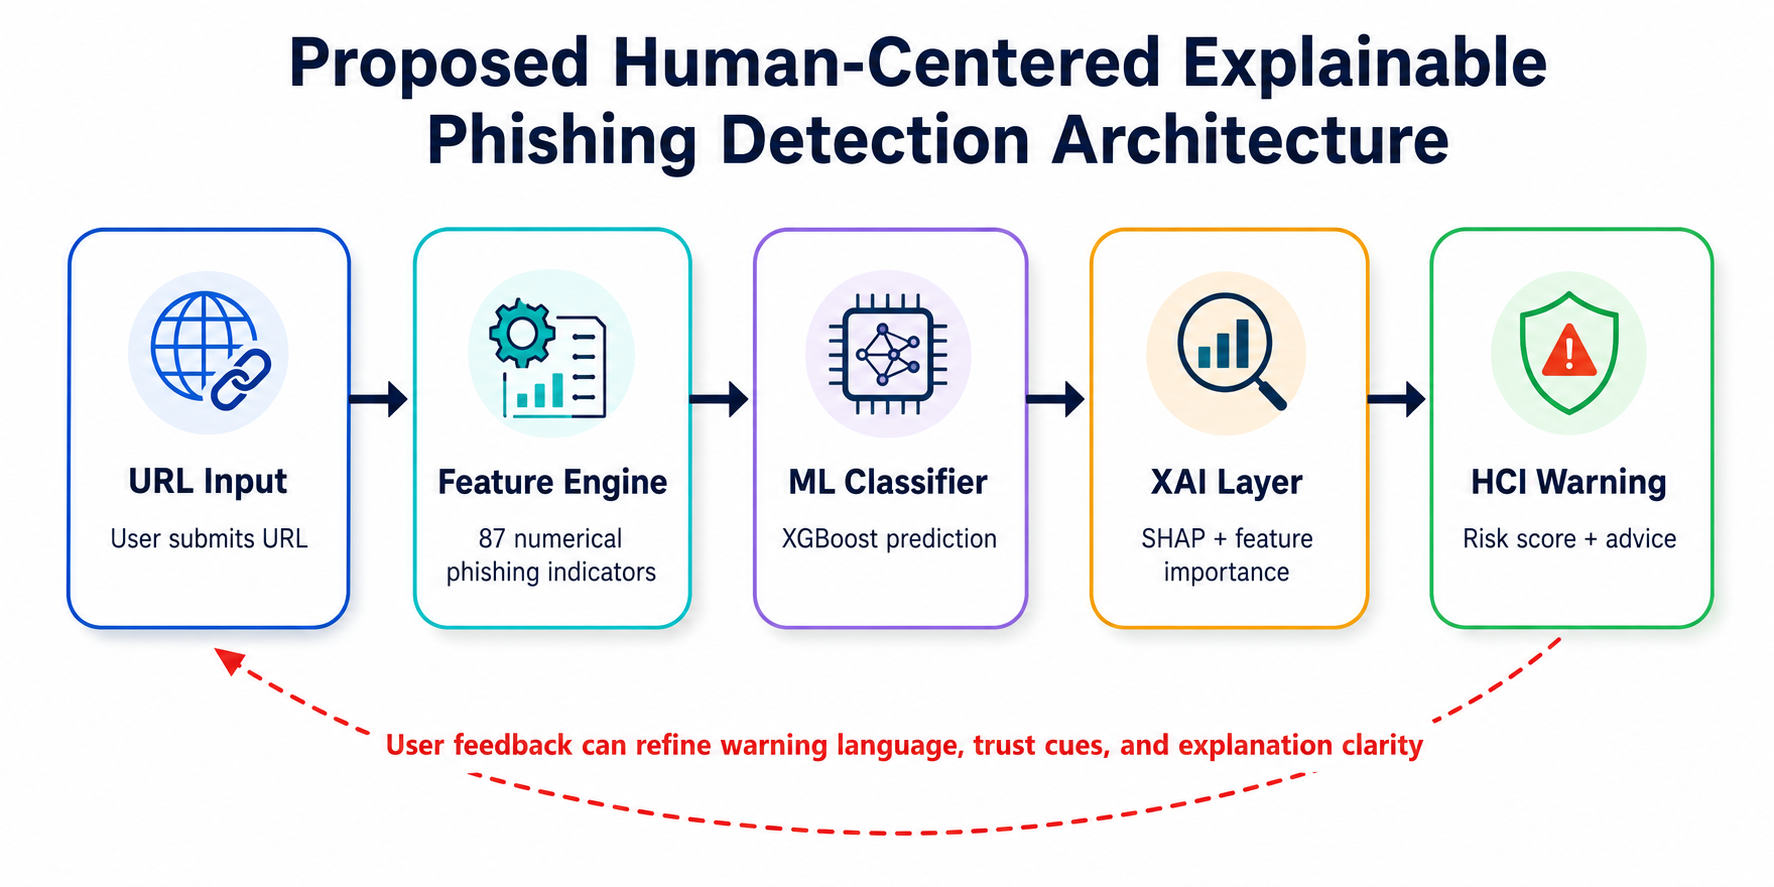
\includegraphics[width=0.92\linewidth]{figure03.png}
\caption{Proposed human-centred explainable phishing-detection framework, integrating the
dataset, modelling pipeline, explainability layer and interface output. Source: Authors'
design.}
\label{fig:framework}
\end{figure}

\begin{figure}[H]\centering
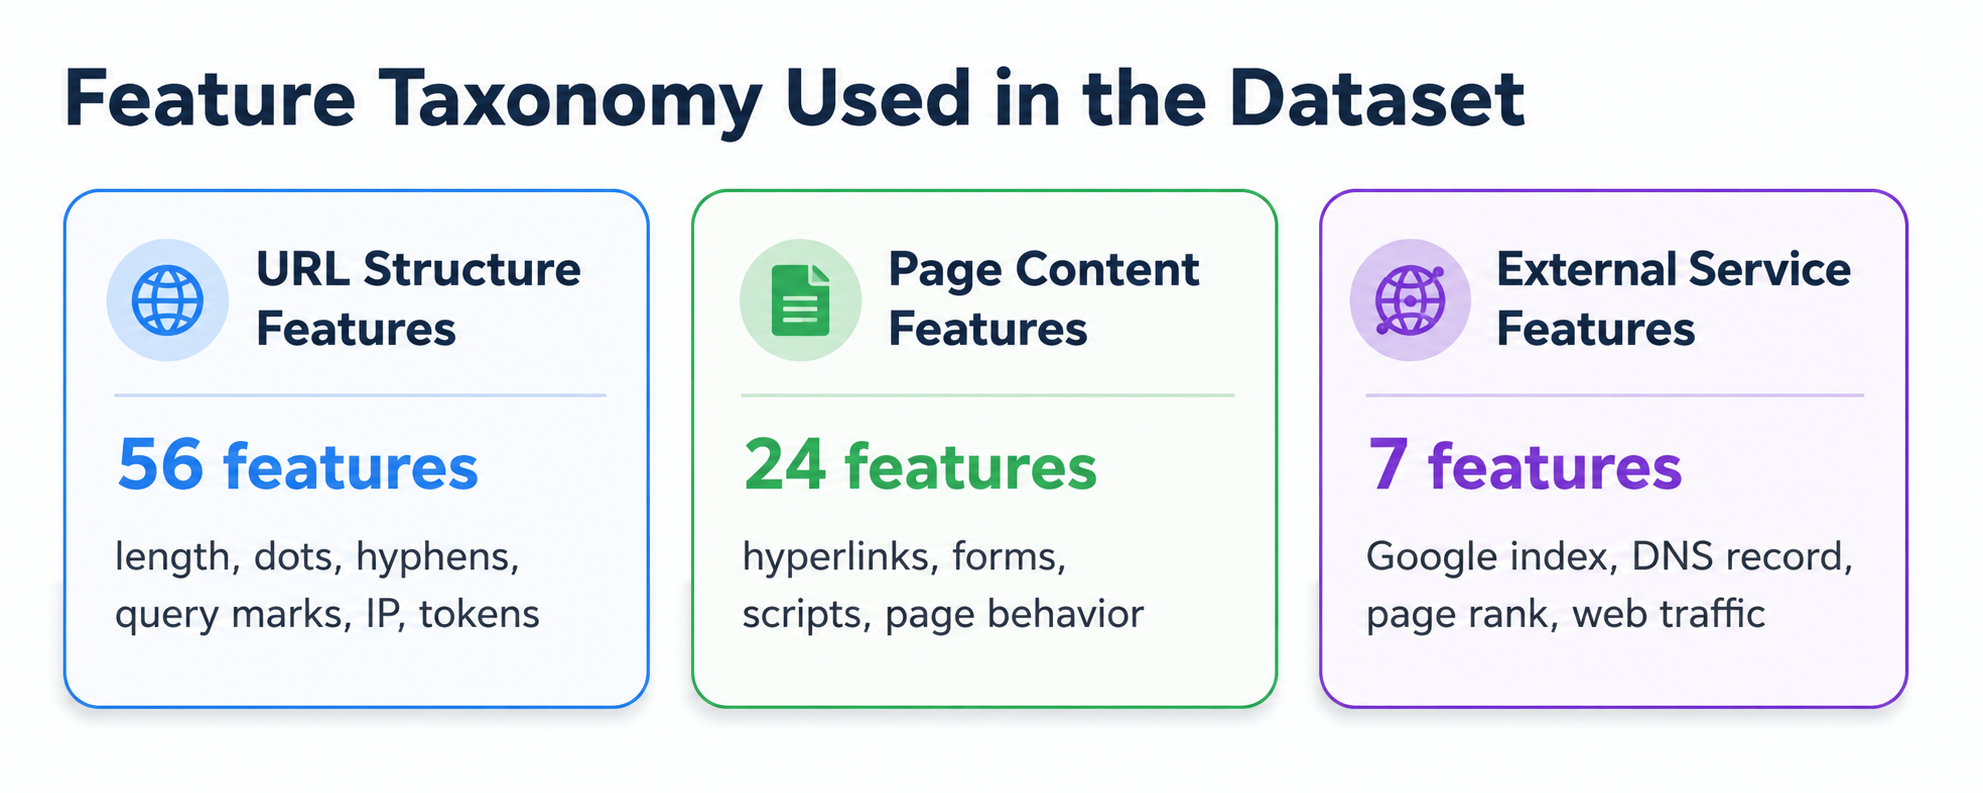
\includegraphics[width=0.92\linewidth]{figure04.png}
\caption{Dataset feature taxonomy: URL-based, page-content and external-service features.
Source: Authors' analysis.}
\label{fig:taxonomy}
\end{figure}

\begin{table}[H]
\caption{Feature categories used in the dataset.}
\label{tab:feature-categories}
\centering\footnotesize
\begin{tabularx}{\textwidth}{p{3.2cm} L L}
\toprule
\textbf{Feature category} & \textbf{Examples} & \textbf{Explanation potential for users} \\
\midrule
URL-based features & length\_url, nb\_dots, nb\_hyphens, nb\_qm, ratio\_digits\_host &
Suspicious URL length, unusual symbols or confusing structure. \\
Page-content features & nb\_hyperlinks, login\_form, iframe, safe\_anchor &
Risky page behaviour and abnormal linking patterns. \\
External-service features & google\_index, page\_rank, web\_traffic, dns\_record, domain\_age &
Weak reputation, missing index signals or low domain trust. \\
\bottomrule
\end{tabularx}
\end{table}

\begin{figure}[H]\centering
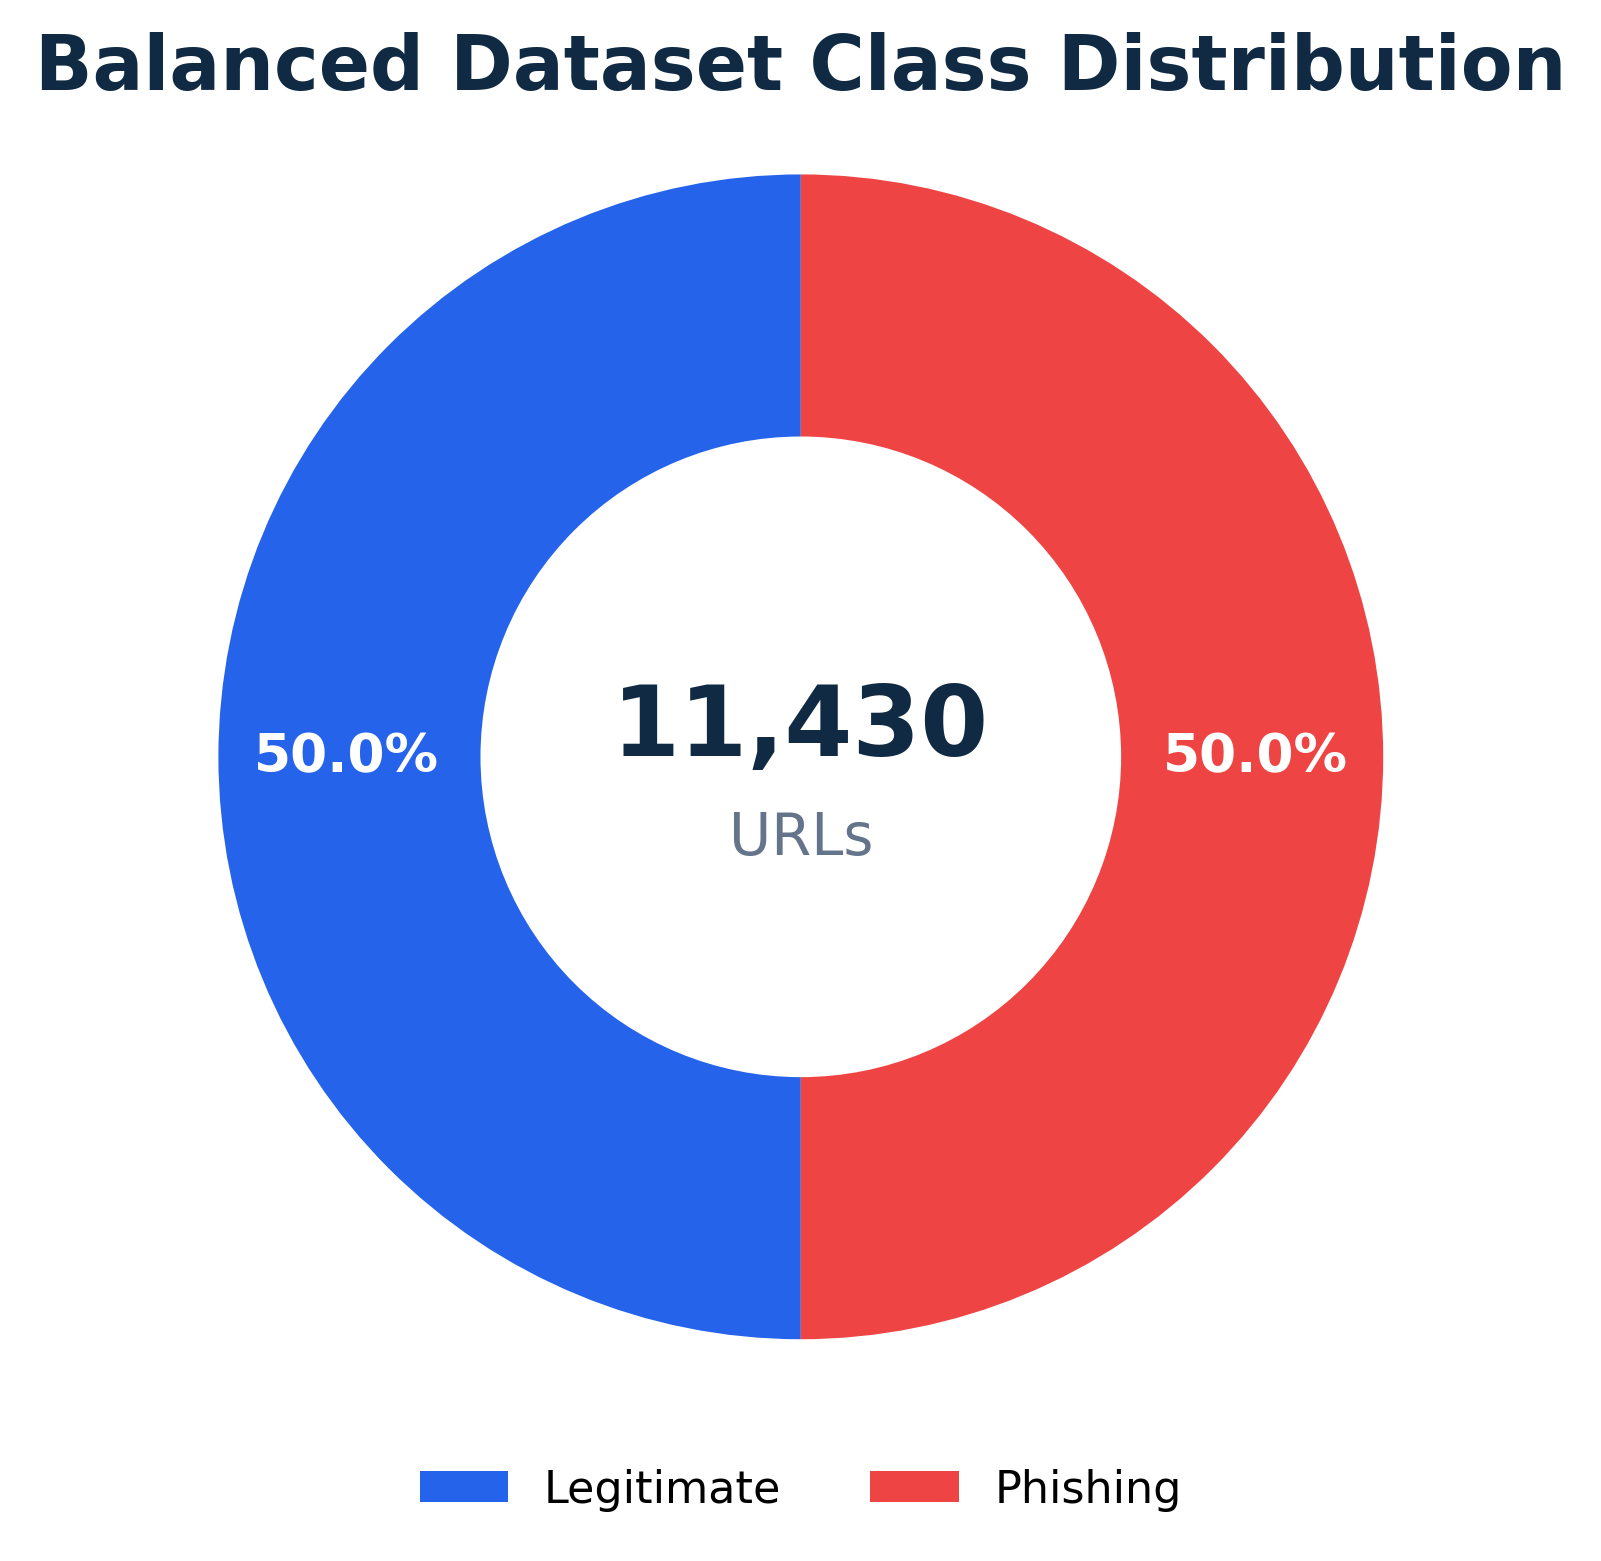
\includegraphics[width=0.75\linewidth]{figure05.png}
\caption{Balanced class distribution of the Web Page Phishing Detection dataset. Source:
Authors' analysis.}
\label{fig:class-dist}
\end{figure}

\subsection{Data Preprocessing}

Using \texttt{pandas}, the data was loaded into Python. The target variable \texttt{status}
was created by assigning 0 for legitimate and 1 for phishing. The raw URL text field was
removed from the modelling matrix, as it is a free-text identifier that could carry
instance-specific information if retained. Data-type, missing-value and invalid-value checks
were performed on the columns; as this dataset was already pre-extracted as numeric features,
no imputation was needed in this analysis. The data was split into an 80--20 train--test set
with stratification to ensure a balanced class distribution in each set (1{,}143 legitimate
and 1{,}143 phishing instances in the test set). A fixed random seed was set to make the split
reproducible.

\textit{Researcher confirmation required: confirm the exact treatment of any missing/duplicate
records, whether feature scaling was applied (and, if so, that it was fitted inside a pipeline
on the training folds only), and the specific random-seed value used for the split and models.}

\subsection{Model Development}

To implement the supervised classifiers, the \texttt{scikit-learn} and \texttt{XGBoost}
libraries were used, with the following classifiers: Logistic Regression, Decision Tree,
Random Forest, Extra Trees, Gradient Boosting and the XGBoost classifier. In this study, no
systematic hyperparameter search (e.g.\ grid or randomised search) was carried out; models
were trained with the default hyperparameters provided by the libraries. This is stated
explicitly as a limitation, as better performance may be achievable after tuning. The focus
for model selection was the F1-score for the phishing class, which reflects the penalty
associated with missed detections.

\textit{Hyperparameters to confirm: if present, confirm exactly what they are; whether
class-weighting was used; and, if tuning was performed, whether it was tuned for each model.}

\subsection{Cross-Validation}

Five-fold stratified cross-validation was used to evaluate the stability of the models, with
the F1-score of the phishing class as the evaluation metric. The cross-validation results are
tabulated as mean and standard deviation over the folds (Table~\ref{tab:cv}). Any
information-dependent preprocessing should be fitted within each training fold, not on the
entire dataset, to prevent leakage.

\subsection{Evaluation Metrics}

The metrics used to measure performance are defined in Table~\ref{tab:metrics}. Of particular
importance in phishing detection are recall and the false-negative rate: a false negative (a
phishing page that is not detected) can leave a user vulnerable to credential theft, while a
false positive (a legitimate page flagged as phishing) is mainly a nuisance and, if frequent,
can cause warning fatigue. Both types of error are therefore reported. For the
precision--recall analysis, the average precision (AP) is reported, which should not be
confused with the ROC-AUC.

\begin{table}[H]
\caption{Evaluation-metric definitions.}
\label{tab:metrics}
\centering\footnotesize
\renewcommand{\arraystretch}{1.8}
\begin{tabularx}{\textwidth}{p{4.2cm} L}
\toprule
\textbf{Metric} & \textbf{Definition} \\
\midrule
Accuracy & $\dfrac{TP+TN}{TP+TN+FP+FN}$ \\
Precision & $\dfrac{TP}{TP+FP}$ \\
Recall (sensitivity) & $\dfrac{TP}{TP+FN}$ \\
F1-score & $\dfrac{2\cdot\text{Precision}\cdot\text{Recall}}{\text{Precision}+\text{Recall}}$ \\
Specificity & $\dfrac{TN}{TN+FP}$ \\
False-positive rate & $\dfrac{FP}{FP+TN}$ \\
False-negative rate & $\dfrac{FN}{FN+TP}$ \\
ROC-AUC & Area under the receiver-operating-characteristic curve \\
Average precision (AP) & Summary of the precision--recall curve \\
\bottomrule
\end{tabularx}
\end{table}

\subsection{Explainability Procedure}

The top-performing model (XGBoost) was chosen for explanation. We employed two complementary
techniques: the model's built-in feature importance for global ranking, and SHAP for global
and local explanations. A positive SHAP value pushes a prediction towards the phishing class;
a negative value pushes it towards the legitimate class. Global explanations summarise feature
effects over multiple instances (SHAP summary plot), while local explanations explain why a
specific decision was made. These technical attributions were then translated into
plain-language statements (e.g.\ a strong negative contribution from \texttt{google\_index}
becomes ``the website has a poor search-engine reputation'') which were presented on the
interface.

\textit{Researcher confirmation required: confirm the type of explainer (TreeExplainer), the
background/reference data, and the sample size used to compute the SHAP values.}

\subsection{Interface Design}

The interface is intended for non-technical users making everyday browsing decisions. The
design requirements were: present a clear prediction label and a numeric risk score; provide a
short, plain-language explanation of the main reasons; offer concrete safety advice; use
colour-coded risk indicators supported by text (so meaning does not depend on colour alone);
avoid technical jargon; and present a clear warning hierarchy. To support trust calibration,
the interface communicates the basis for the warning rather than asserting certainty, so users
can judge how far to rely on it. The interface is a static mock-up (Figure~\ref{fig:mockup})
and was not implemented as working software.

\subsection{Software and Reproducibility}

The experiments were conducted in Python using \texttt{pandas}, \texttt{NumPy},
\texttt{scikit-learn}, \texttt{XGBoost}, \texttt{SHAP} and \texttt{Matplotlib}. Exact library
versions are not recorded in the available materials and are left as placeholders below, to be
completed by the researcher; they are not invented here.

\begin{itemize}[noitemsep,topsep=2pt]
\item Python
\item pandas / NumPy
\item scikit-learn
\item XGBoost
\item SHAP
\item Matplotlib
\end{itemize}

The trained model and result files (\texttt{best\_phishing\_detection\_model.pkl},
\texttt{model\_performance\_results.csv}, \texttt{cross\_validation\_results.csv},
\texttt{feature\_importance\_results.csv}, and the figure set) are available with the project
and support reproduction of the reported results.

%================================ 5. RESULTS =================================
\section{Results and Statistical Analysis}

\subsection{Model Performance}

The six classifiers were compared on the held-out test set (Table~\ref{tab:performance}).
XGBoost achieved the strongest overall performance, with an accuracy of 0.96632, precision of
0.96187, recall of 0.97113, F1-score of 0.96648 and ROC-AUC of 0.99443. Extra Trees and Random
Forest followed closely, confirming that tree-based ensembles are well suited to this
structured dataset, while Logistic Regression and a single Decision Tree were the weakest. The
high recall of XGBoost is desirable here because it corresponds to few missed phishing pages.

\begin{table}[H]
\caption{Model performance comparison on the held-out test set.}
\label{tab:performance}
\centering\footnotesize
\begin{tabular}{lccccc}
\toprule
\textbf{Model} & \textbf{Accuracy} & \textbf{Precision} & \textbf{Recall} & \textbf{F1-score} & \textbf{ROC-AUC} \\
\midrule
XGBoost             & 0.96632 & 0.96187 & 0.97113 & 0.96648 & 0.99443 \\
Extra Trees         & 0.96457 & 0.96416 & 0.96500 & 0.96458 & 0.99298 \\
Random Forest       & 0.96194 & 0.95833 & 0.96588 & 0.96209 & 0.99355 \\
Gradient Boosting   & 0.95319 & 0.94965 & 0.95713 & 0.95338 & 0.99049 \\
Logistic Regression & 0.93613 & 0.93921 & 0.93263 & 0.93591 & 0.98142 \\
Decision Tree       & 0.93395 & 0.92907 & 0.93963 & 0.93432 & 0.93395 \\
\bottomrule
\end{tabular}
\end{table}

\noindent\footnotesize\textit{Note: precision, recall and F1-score are reported for the
phishing class. All values are rounded to five decimal places.}\normalsize

\begin{figure}[H]\centering
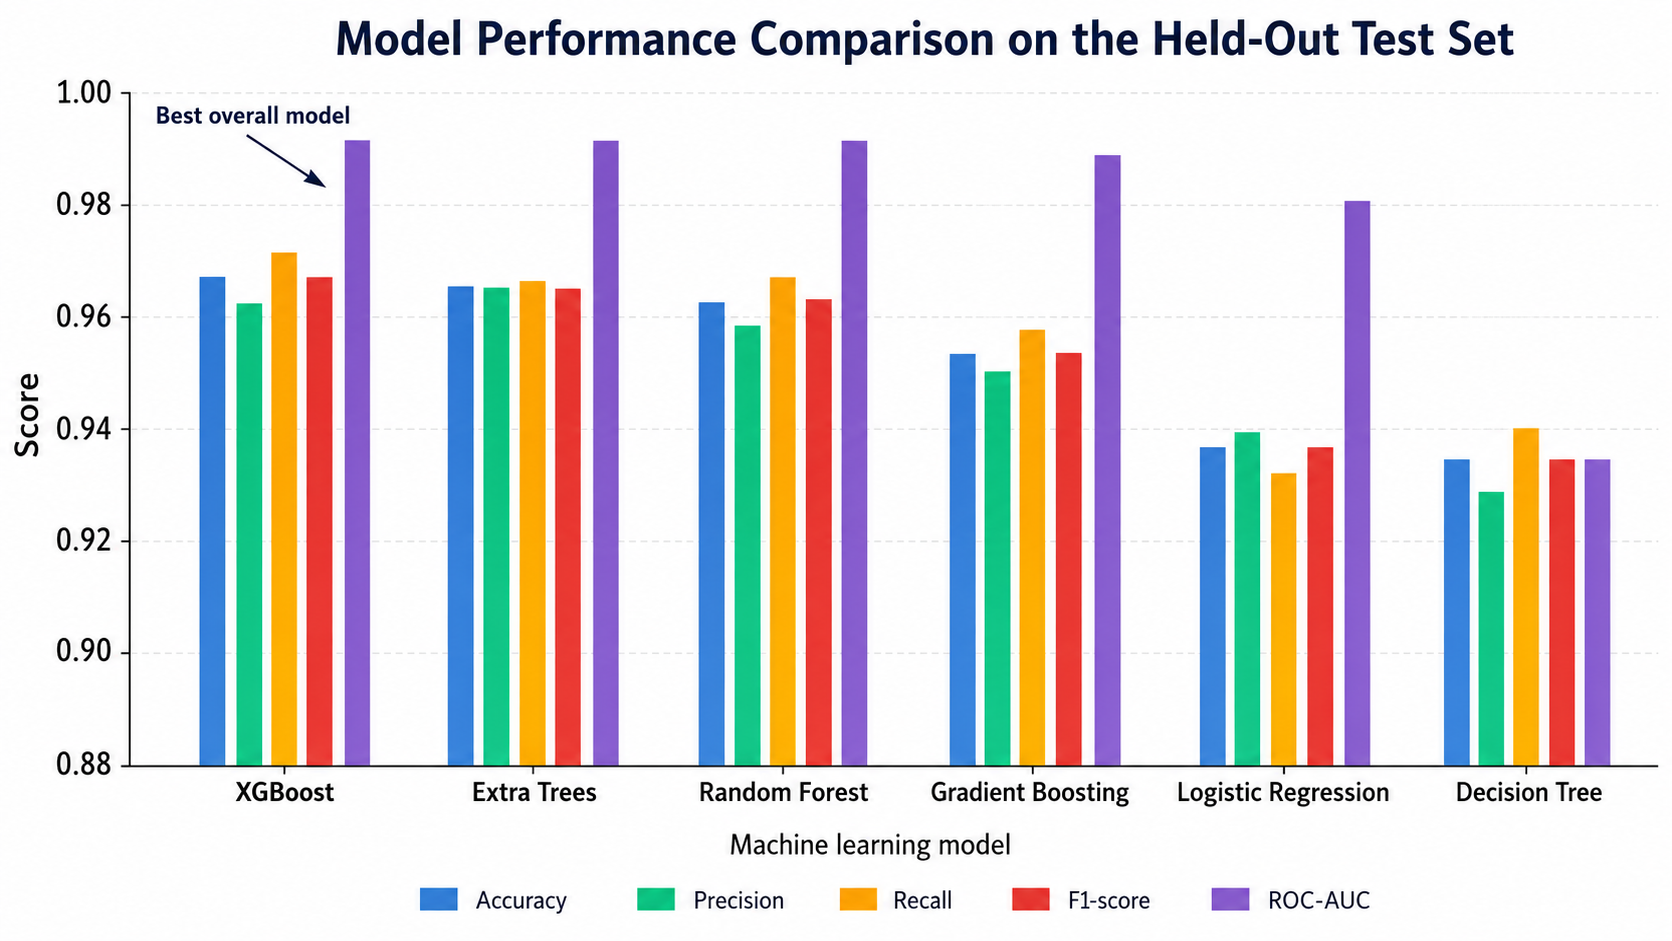
\includegraphics[width=0.9\linewidth]{figure06.png}
\caption{Model performance comparison across all metrics (accuracy, precision, recall,
F1-score and ROC-AUC) on the held-out test set, with XGBoost as the best overall model.
Source: Authors' analysis.}
\label{fig:perf-all}
\end{figure}

\begin{figure}[H]\centering
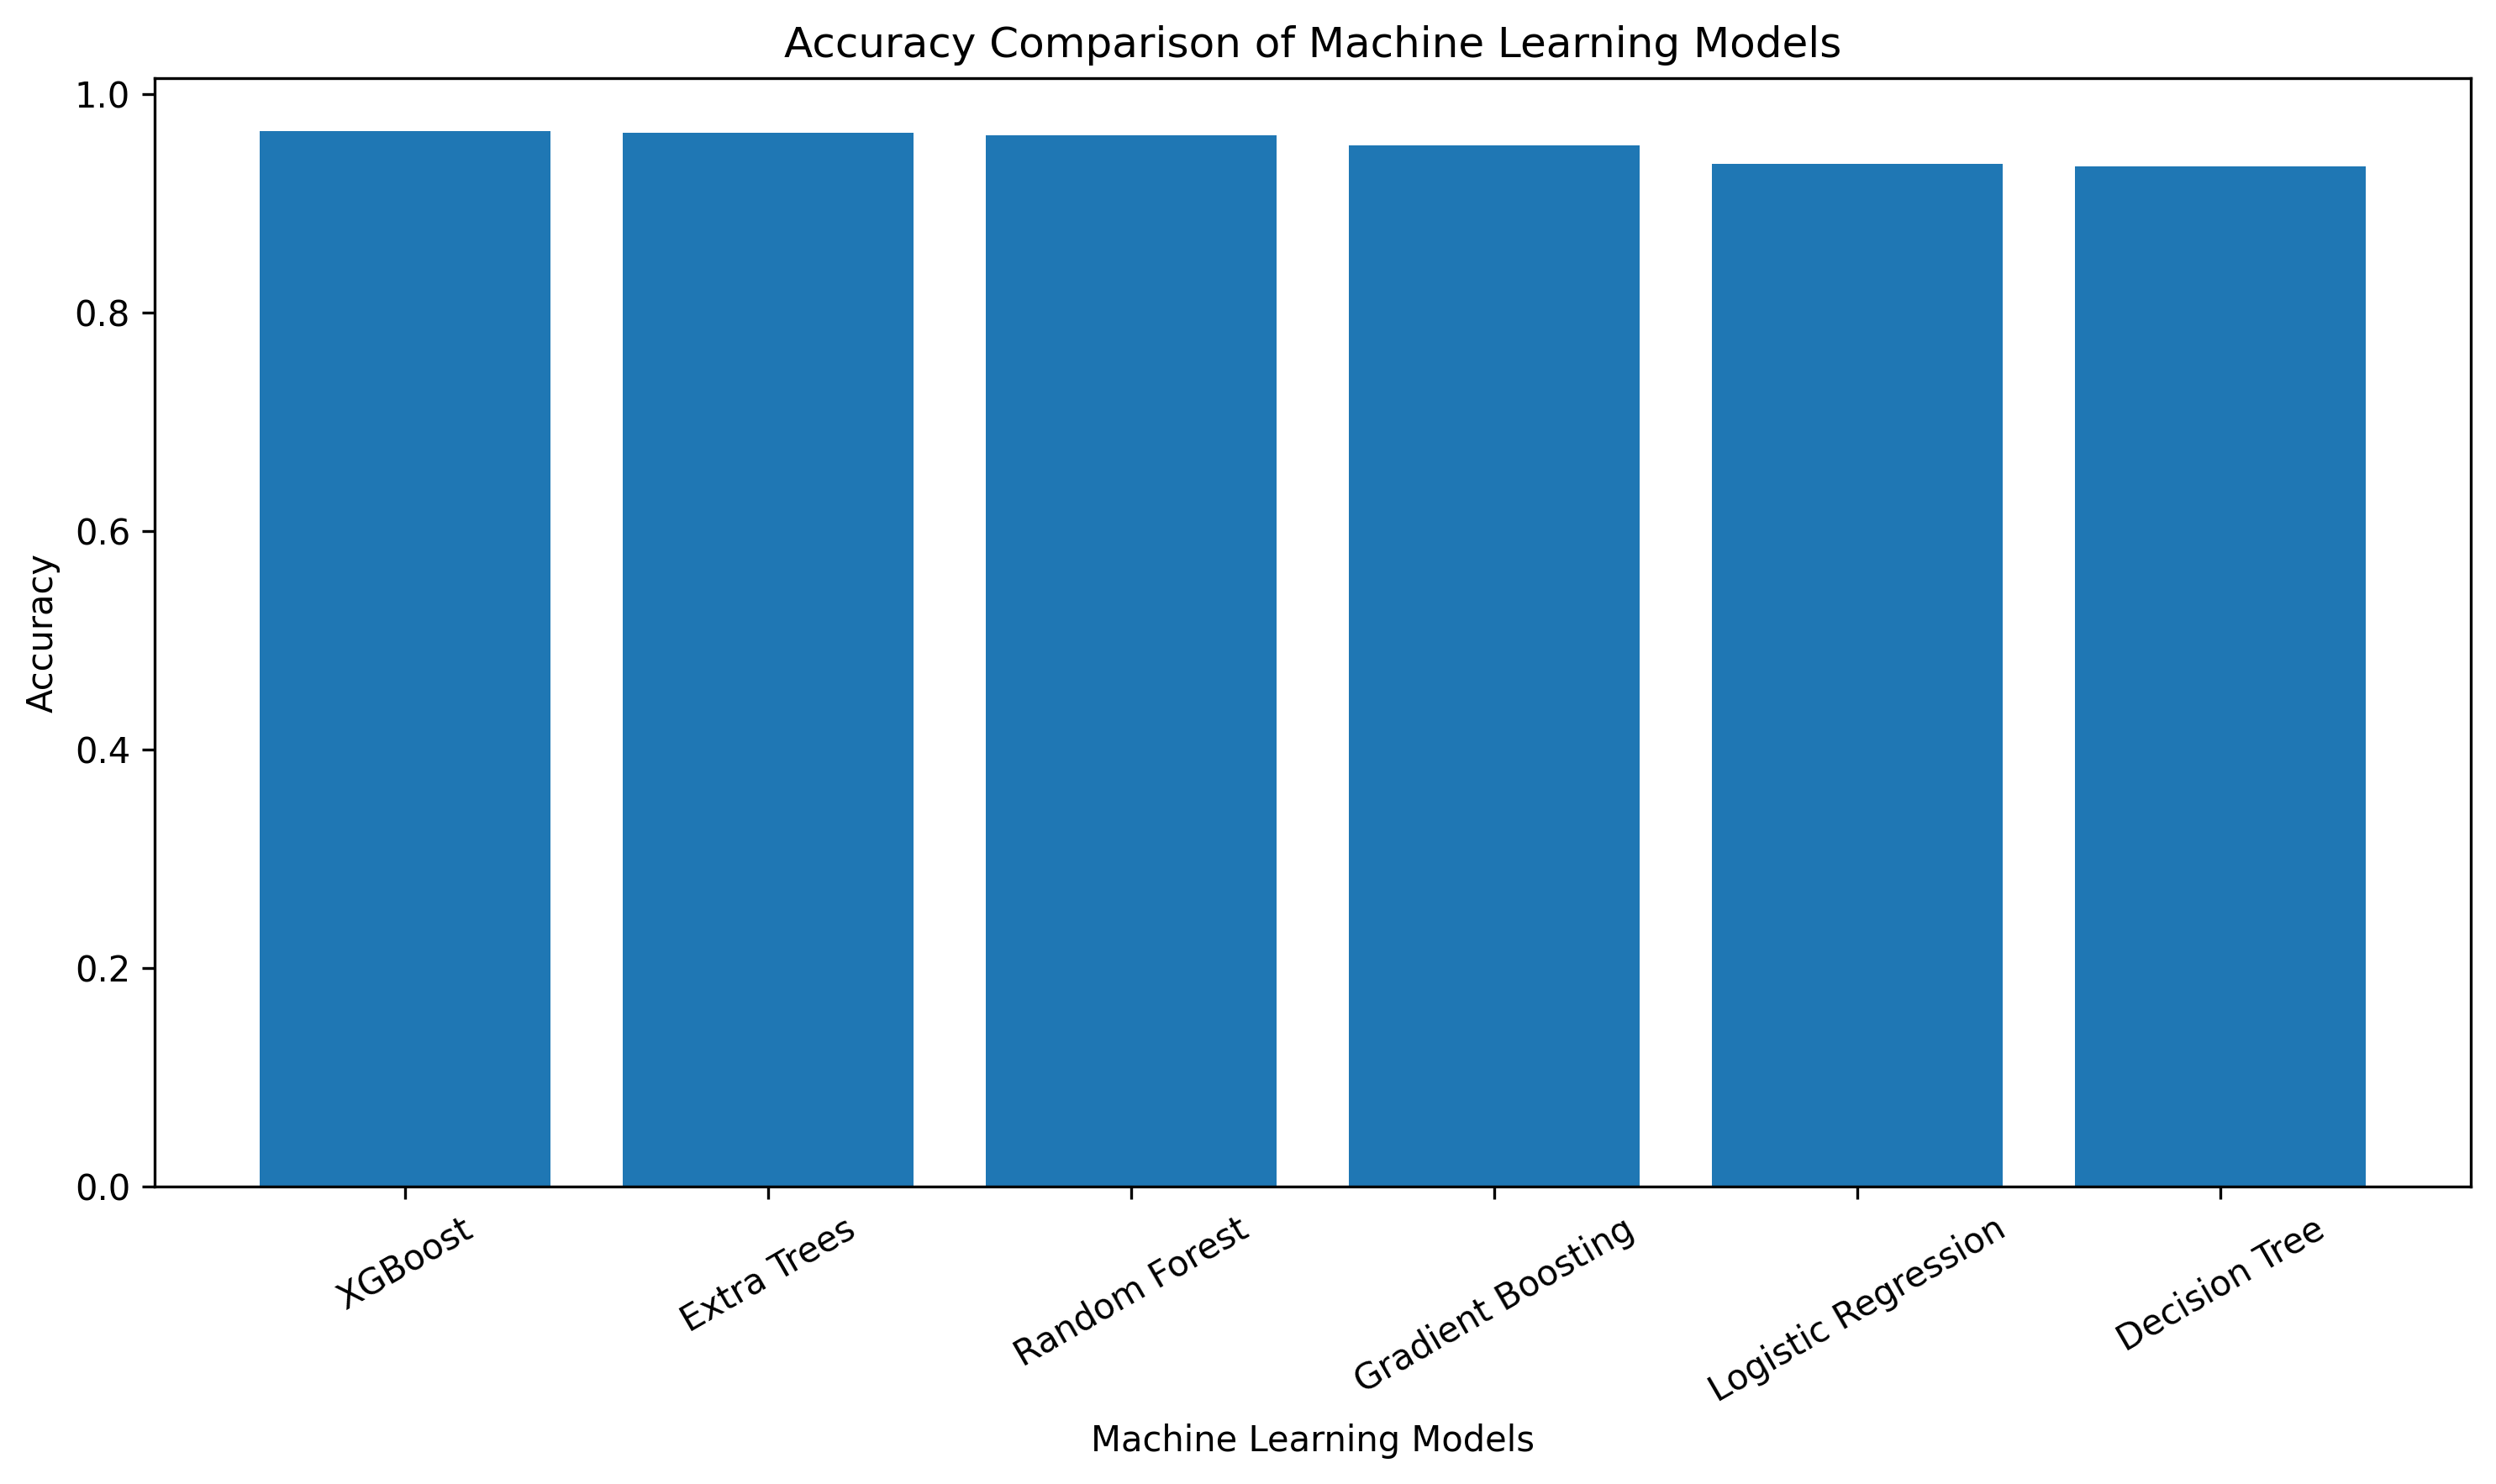
\includegraphics[width=0.7\linewidth]{figure07.png}
\caption{Model accuracy comparison. Source: Authors' analysis.}
\label{fig:acc}
\end{figure}

\begin{figure}[H]\centering
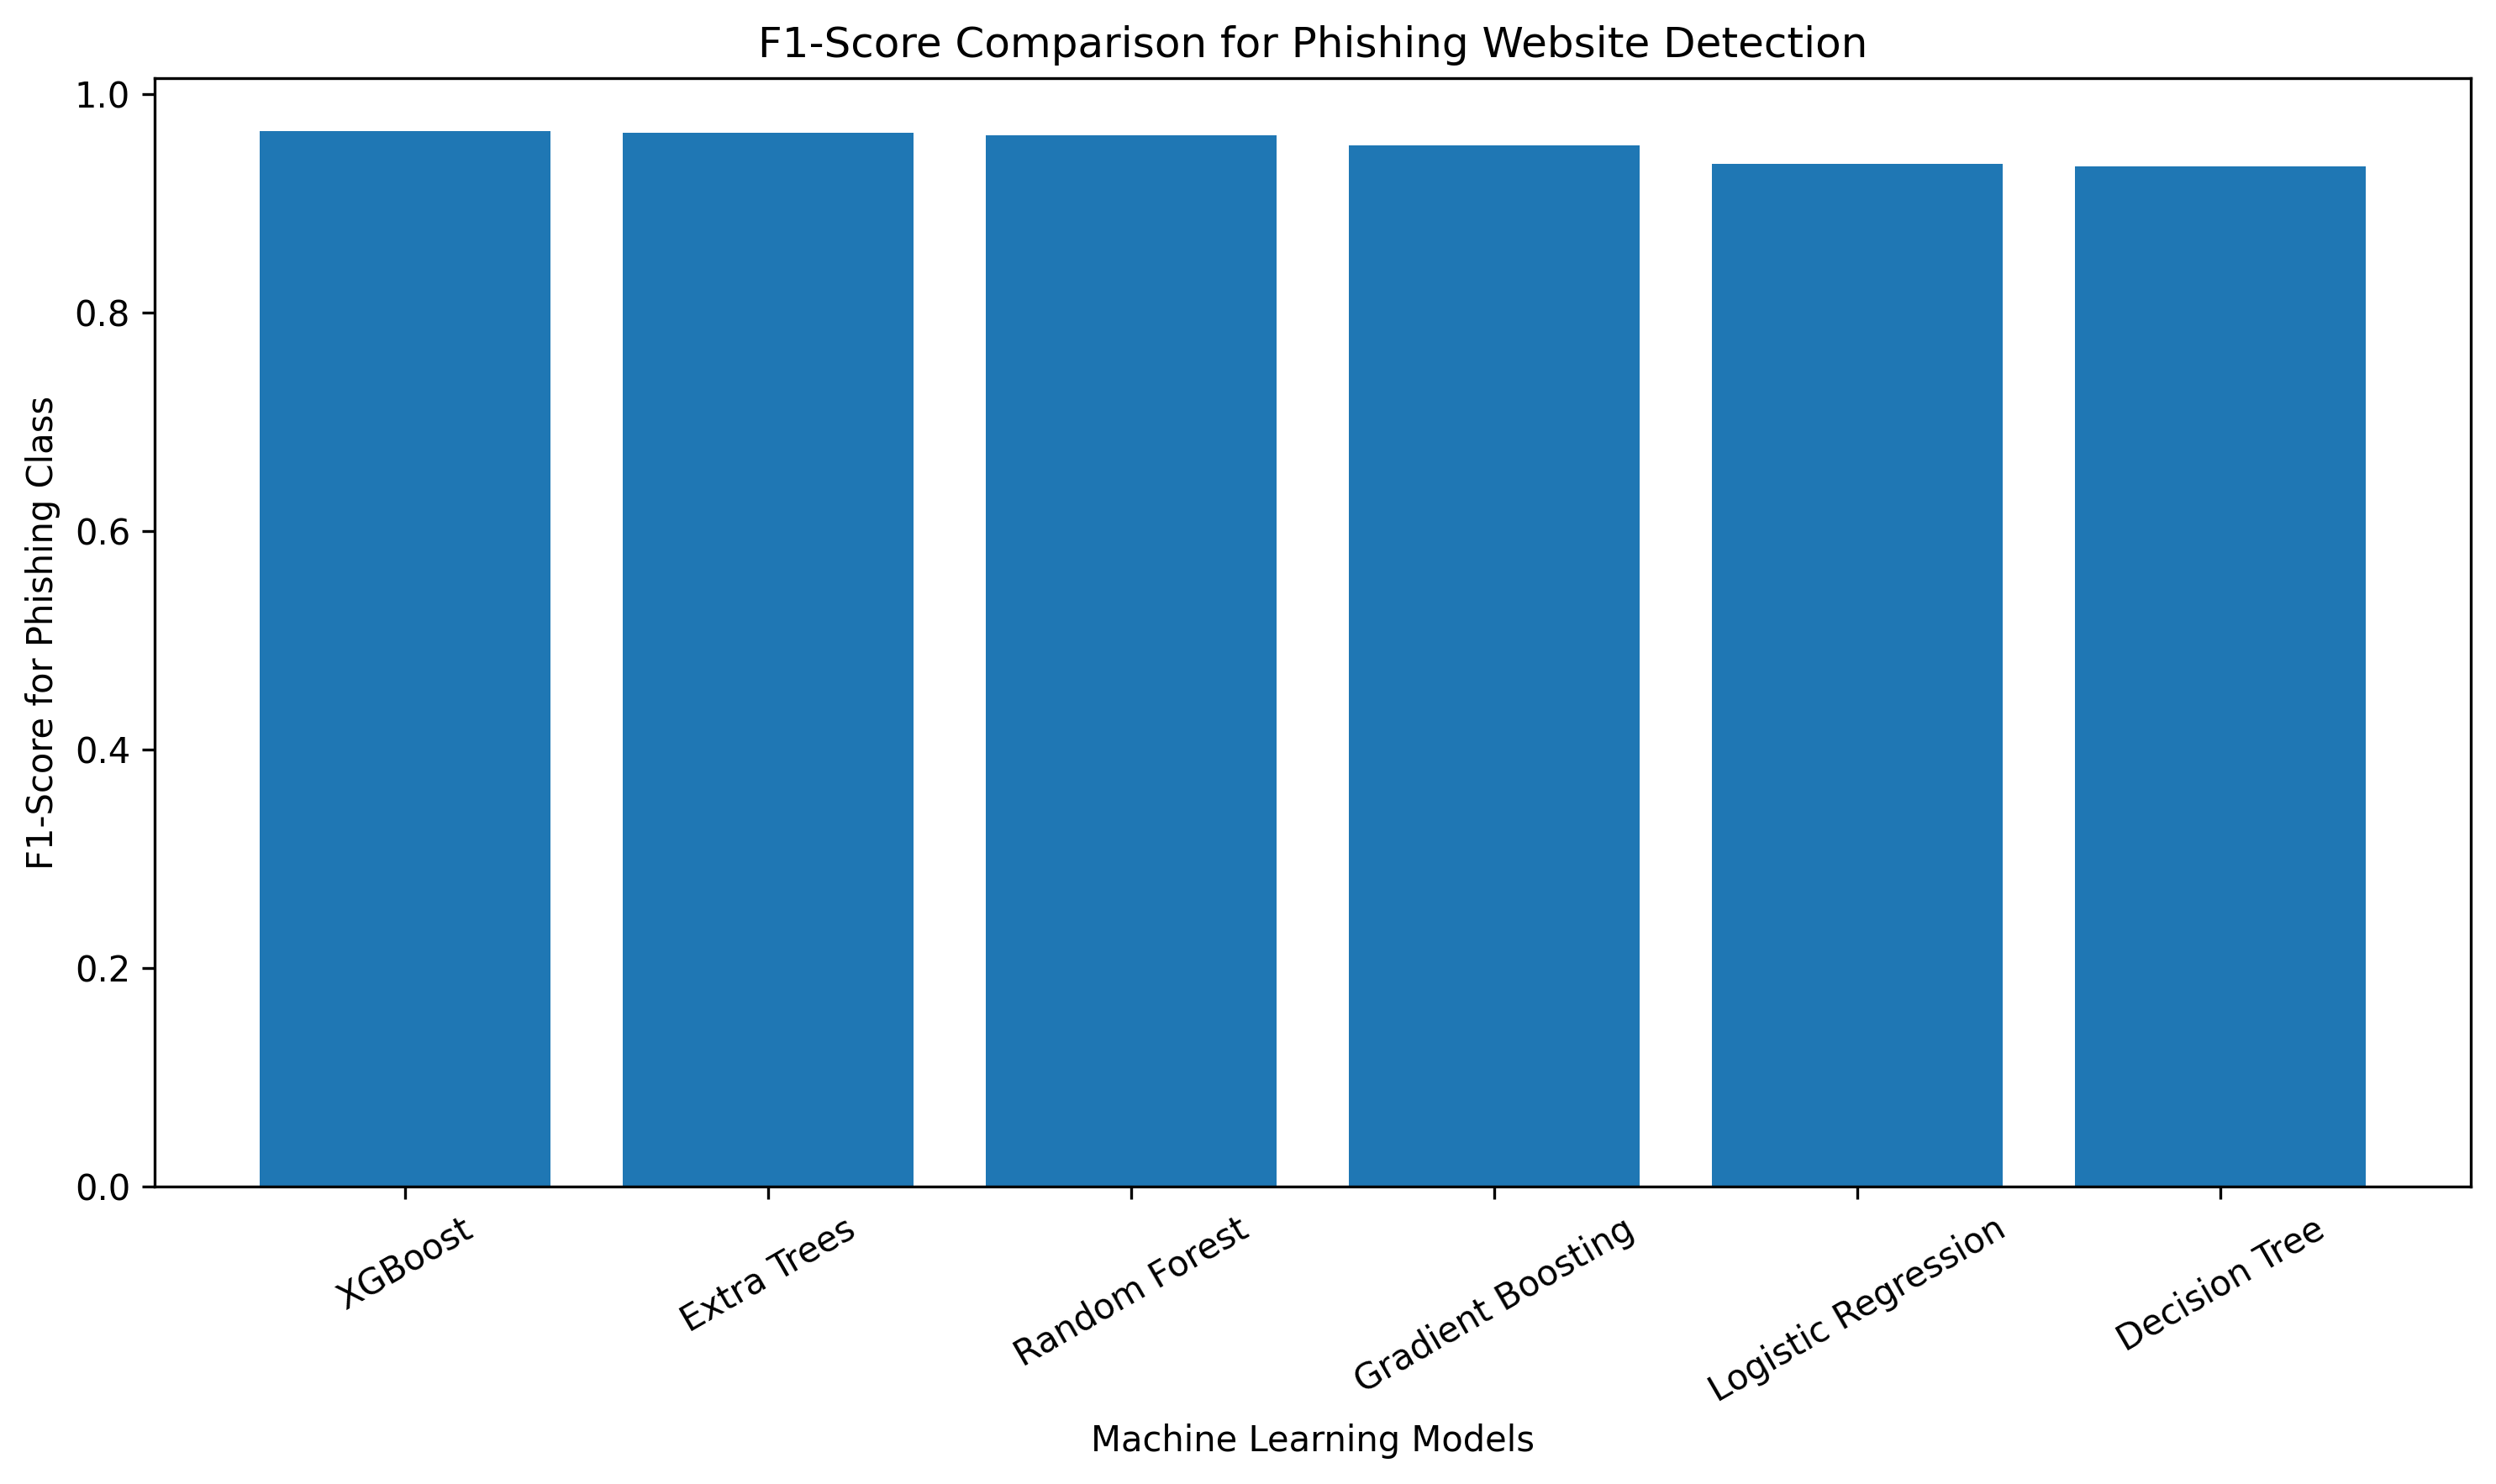
\includegraphics[width=0.7\linewidth]{figure08.png}
\caption{Model F1-score comparison. Source: Authors' analysis.}
\label{fig:f1}
\end{figure}

\begin{figure}[H]\centering
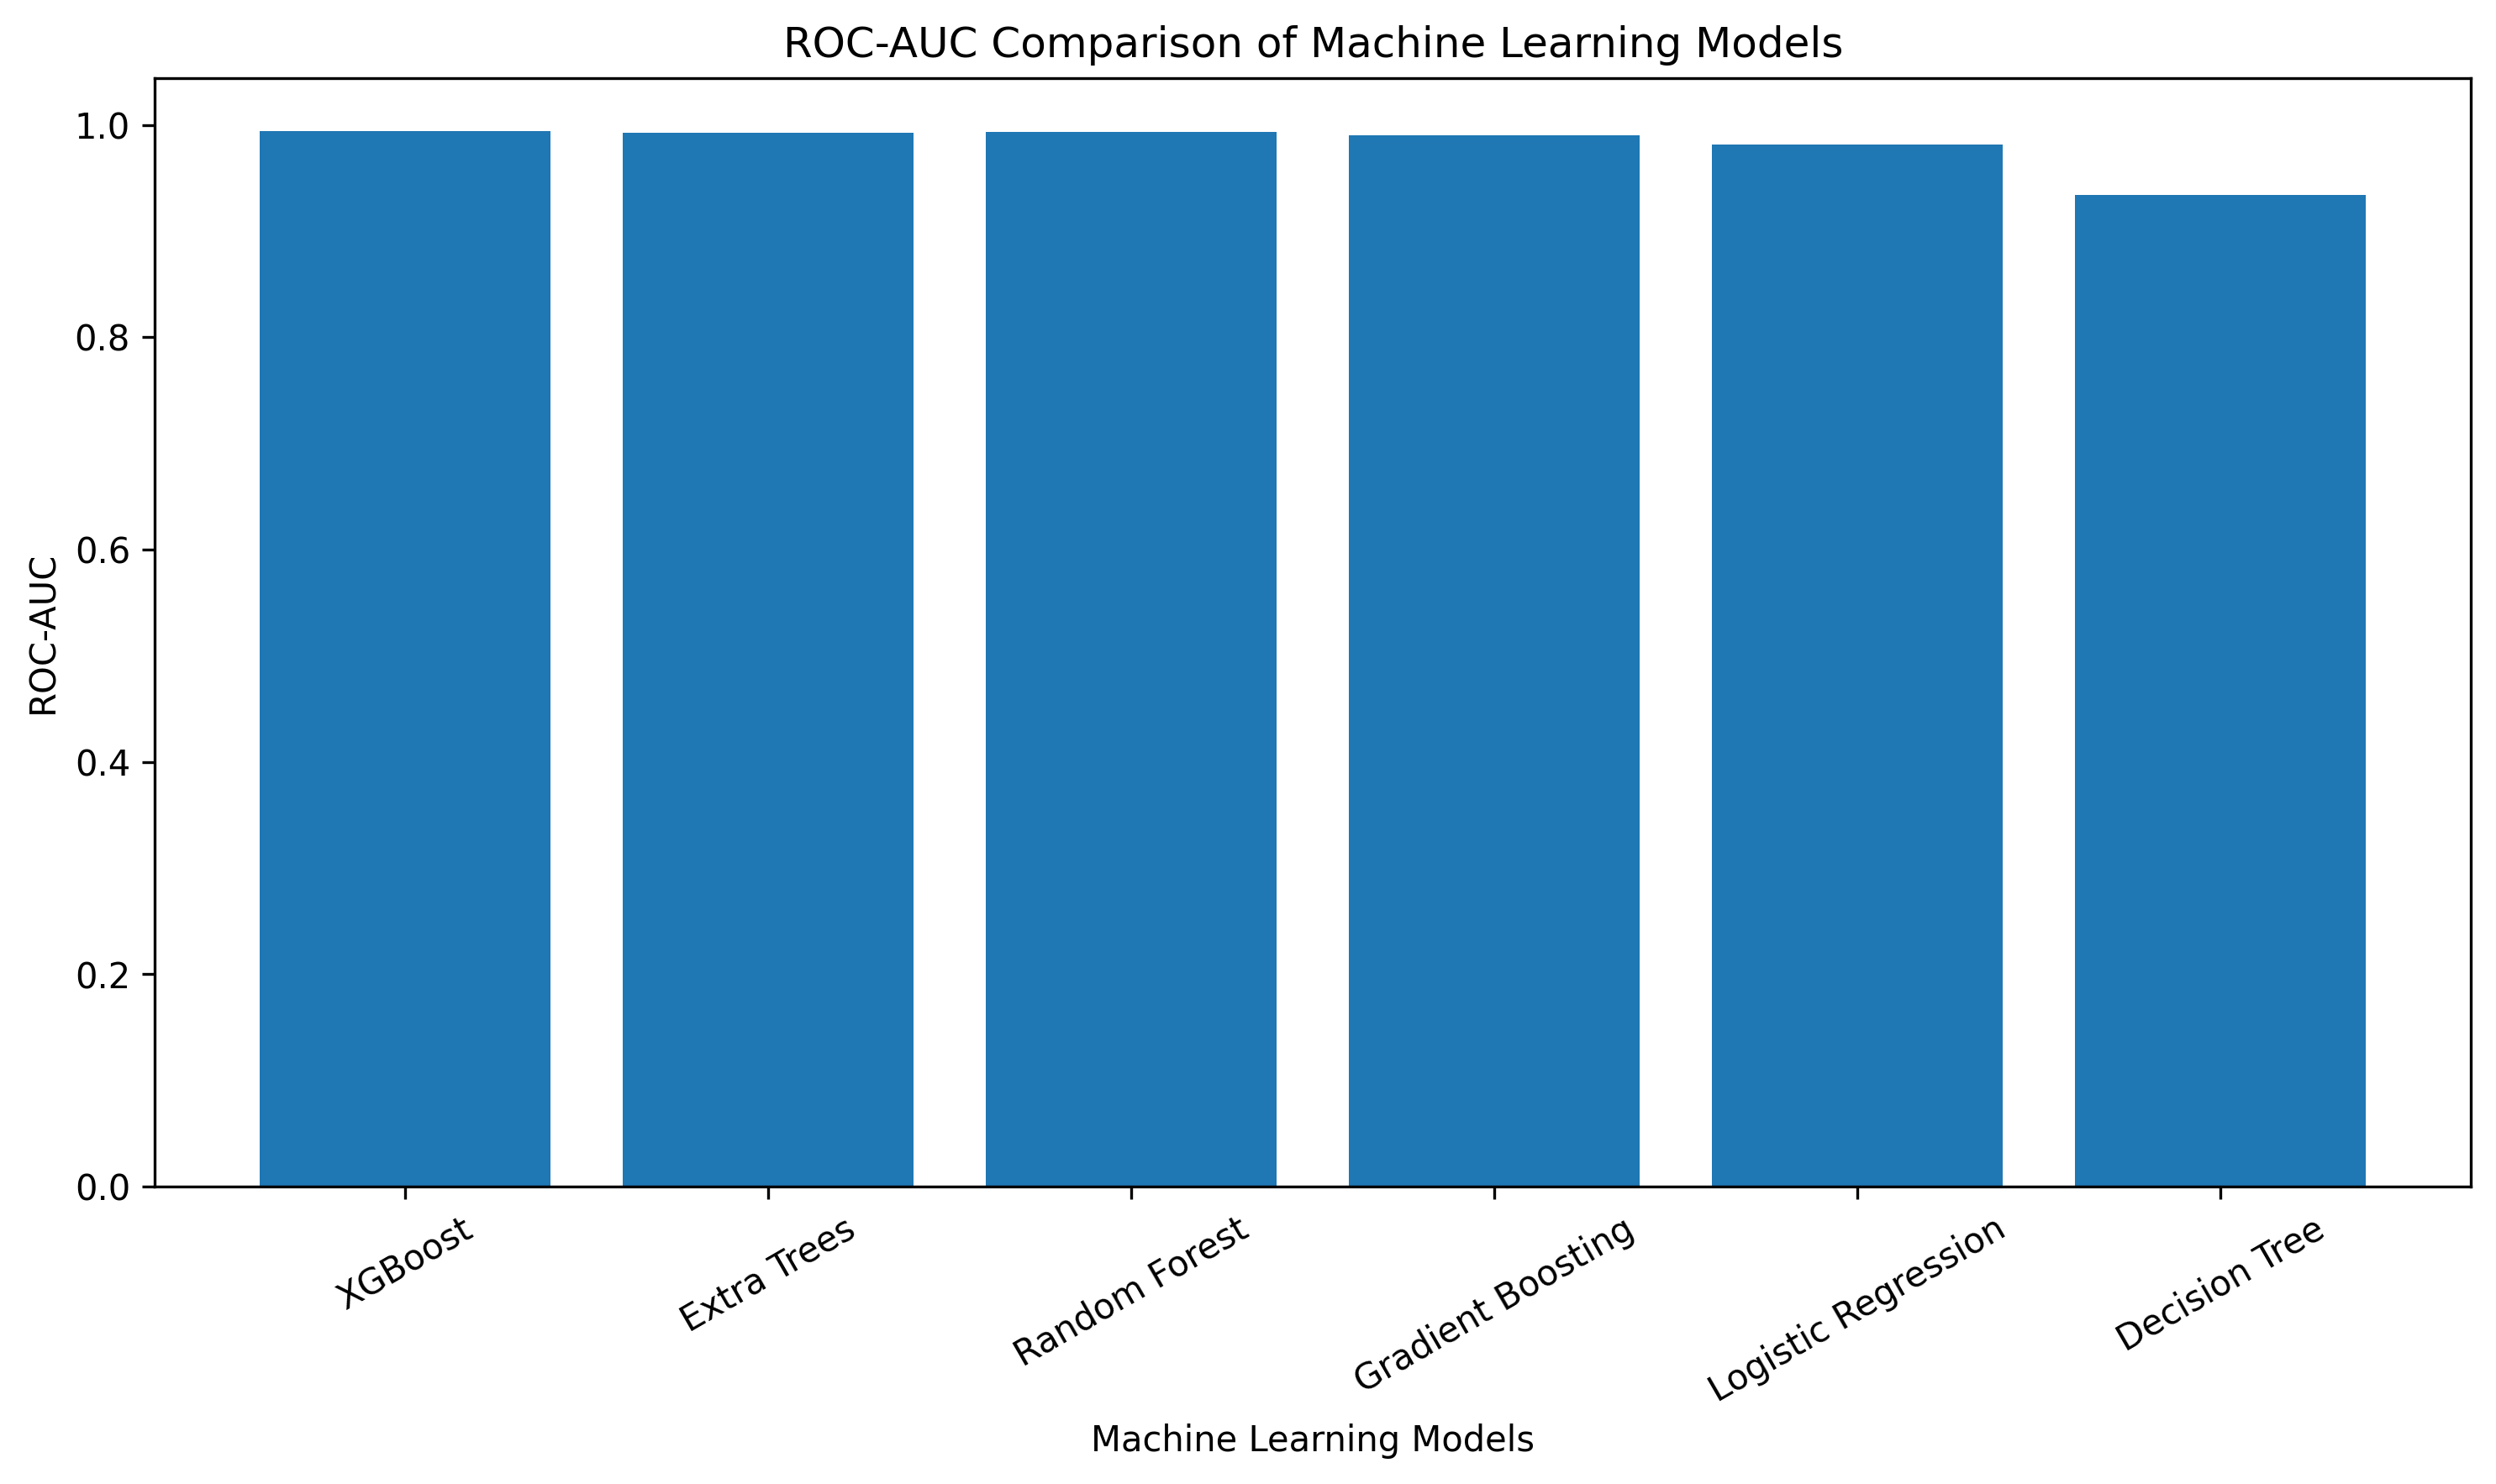
\includegraphics[width=0.7\linewidth]{figure09.png}
\caption{Model ROC-AUC comparison. Source: Authors' analysis.}
\label{fig:rocauc}
\end{figure}

\subsection{Cross-Validation Stability}

Five-fold stratified cross-validation confirmed that the leading models are stable across folds
(Table~\ref{tab:cv}). XGBoost achieved a mean cross-validated F1-score of 0.96906 with a
standard deviation of 0.00202---the highest mean and the smallest variability of the three top
models---indicating consistent performance rather than a result that depends on a single
fortunate split.

\begin{table}[H]
\caption{Cross-validation statistics for the top models.}
\label{tab:cv}
\centering\footnotesize
\begin{tabular}{lcc}
\toprule
\textbf{Model} & \textbf{Mean CV F1-score} & \textbf{SD of CV F1-score} \\
\midrule
XGBoost       & 0.96906 & 0.00202 \\
Random Forest & 0.96705 & 0.00461 \\
Extra Trees   & 0.96341 & 0.00455 \\
\bottomrule
\end{tabular}
\end{table}

\begin{figure}[H]\centering
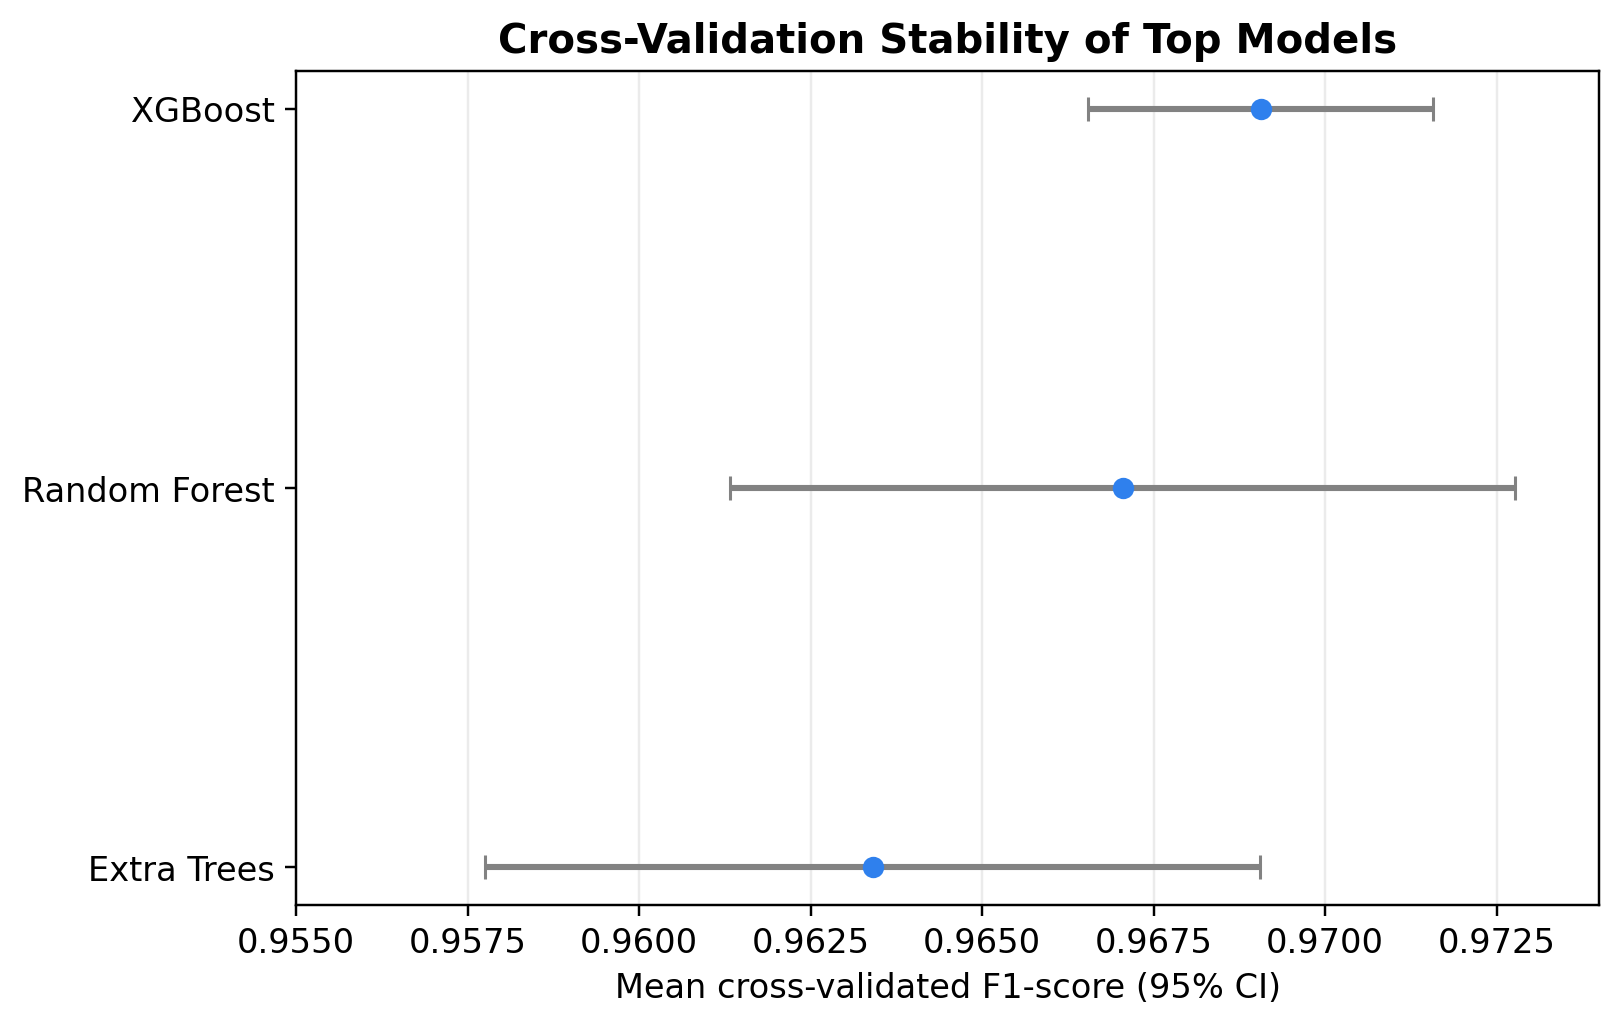
\includegraphics[width=0.7\linewidth]{figure10.png}
\caption{Cross-validation stability of the top models (mean F1-score with standard deviation).
Source: Authors' analysis.}
\label{fig:cv}
\end{figure}

\subsection{Confusion-Matrix Analysis}

On the test set (2{,}286 pages), XGBoost correctly classified 1{,}099 legitimate pages and
1{,}110 phishing pages, with 44 false positives and 33 false negatives
(Figure~\ref{fig:confusion}). The statistics in Table~\ref{tab:confusion} are internally
consistent with the headline metrics in Table~\ref{tab:performance}: accuracy, precision,
recall and F1-score all derive from these four counts. The most security-relevant value is the
2.89\% false-negative rate---the proportion of phishing pages the model misses; the 3.85\%
false-positive rate is less harmful but, if frequent, can lead to warning fatigue.

\begin{table}[H]
\caption{Confusion-matrix-derived statistics for the XGBoost model.}
\label{tab:confusion}
\centering\footnotesize
\begin{tabularx}{\textwidth}{p{3.4cm} c L}
\toprule
\textbf{Statistic} & \textbf{Value} & \textbf{Interpretation} \\
\midrule
True negatives & 1{,}099 & Legitimate websites correctly classified. \\
False positives & 44 & Legitimate websites incorrectly flagged as phishing. \\
False negatives & 33 & Phishing websites missed by the model. \\
True positives & 1{,}110 & Phishing websites correctly detected. \\
Specificity & 0.96150 & Proportion of legitimate sites correctly identified. \\
False-positive rate & 3.85\% & Potential warning-fatigue risk. \\
False-negative rate & 2.89\% & Potential security-exposure risk. \\
\bottomrule
\end{tabularx}
\end{table}

\begin{figure}[H]\centering
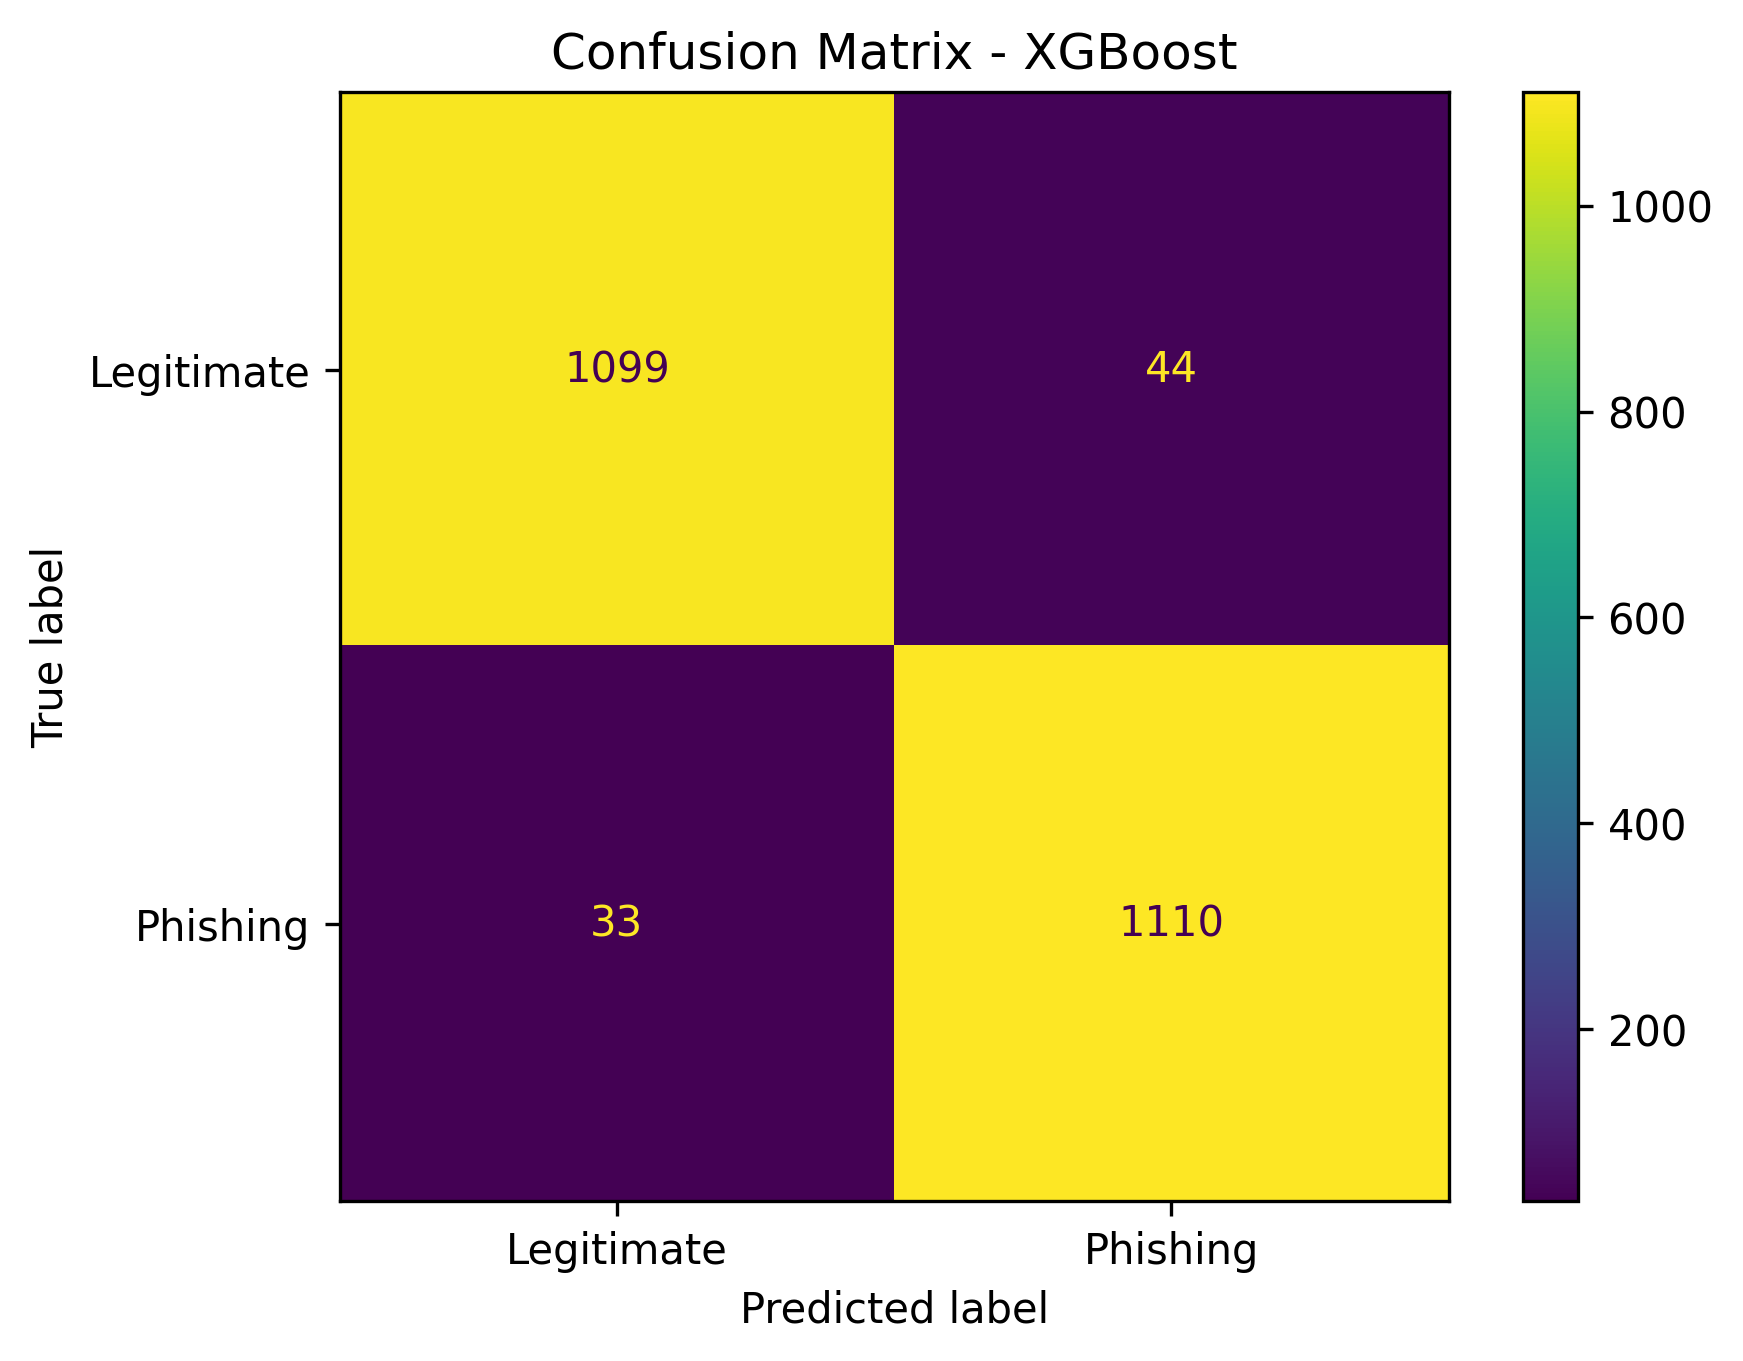
\includegraphics[width=0.6\linewidth]{figure11.png}
\caption{Confusion matrix for the XGBoost model on the test set. Source: Authors' analysis.}
\label{fig:confusion}
\end{figure}

\subsection{ROC and Precision--Recall Analysis}

The ROC curve (Figure~\ref{fig:roc}) shows that the model separates the two classes well across
thresholds, consistent with the ROC-AUC of 0.99443. The precision--recall curve
(Figure~\ref{fig:pr}) summarises performance for the phishing (positive) class and reports an
average precision of around 0.99. As the dataset is balanced, the ROC and precision--recall
analyses tell essentially the same story here, although the average precision is a different
quantity from the ROC-AUC and is reported separately.

\textit{Researcher confirmation required: record the actual average-precision value from the
notebook (rounded to two decimal places).}

\begin{figure}[H]\centering
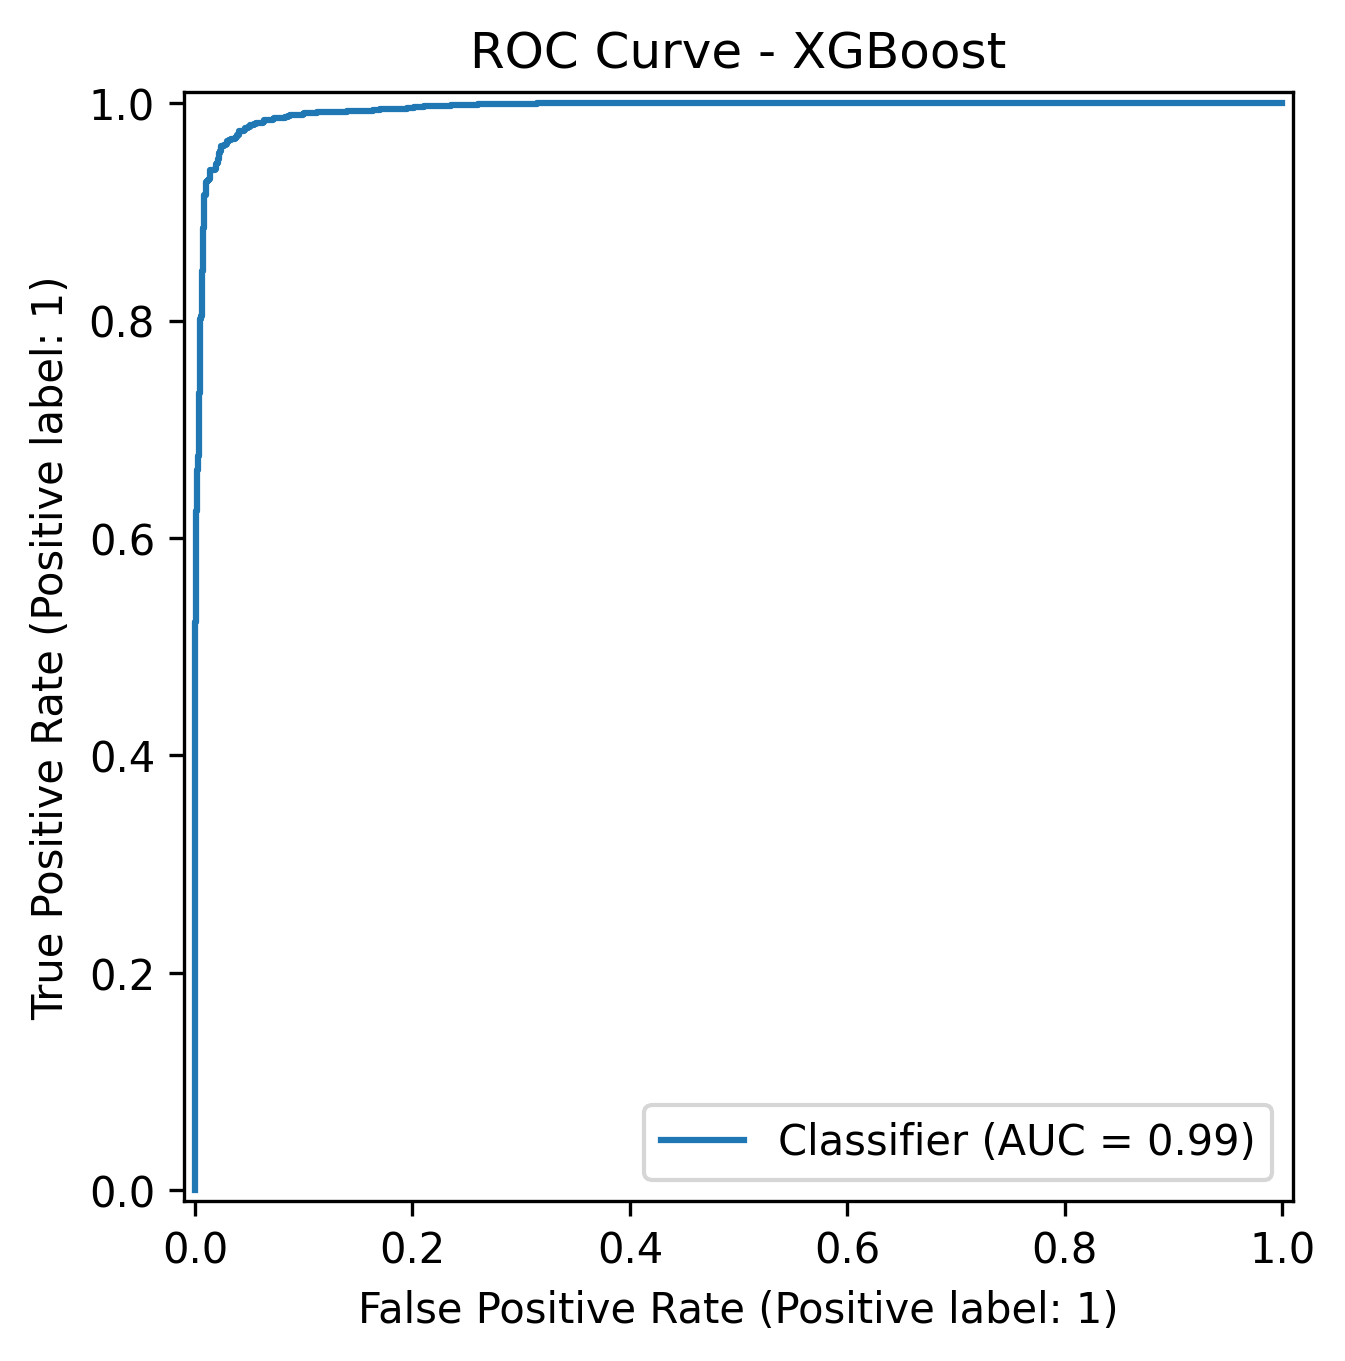
\includegraphics[width=0.65\linewidth]{figure12.png}
\caption{ROC curve for the XGBoost model (AUC $\approx$ 0.99). Source: Authors' analysis.}
\label{fig:roc}
\end{figure}

\begin{figure}[H]\centering
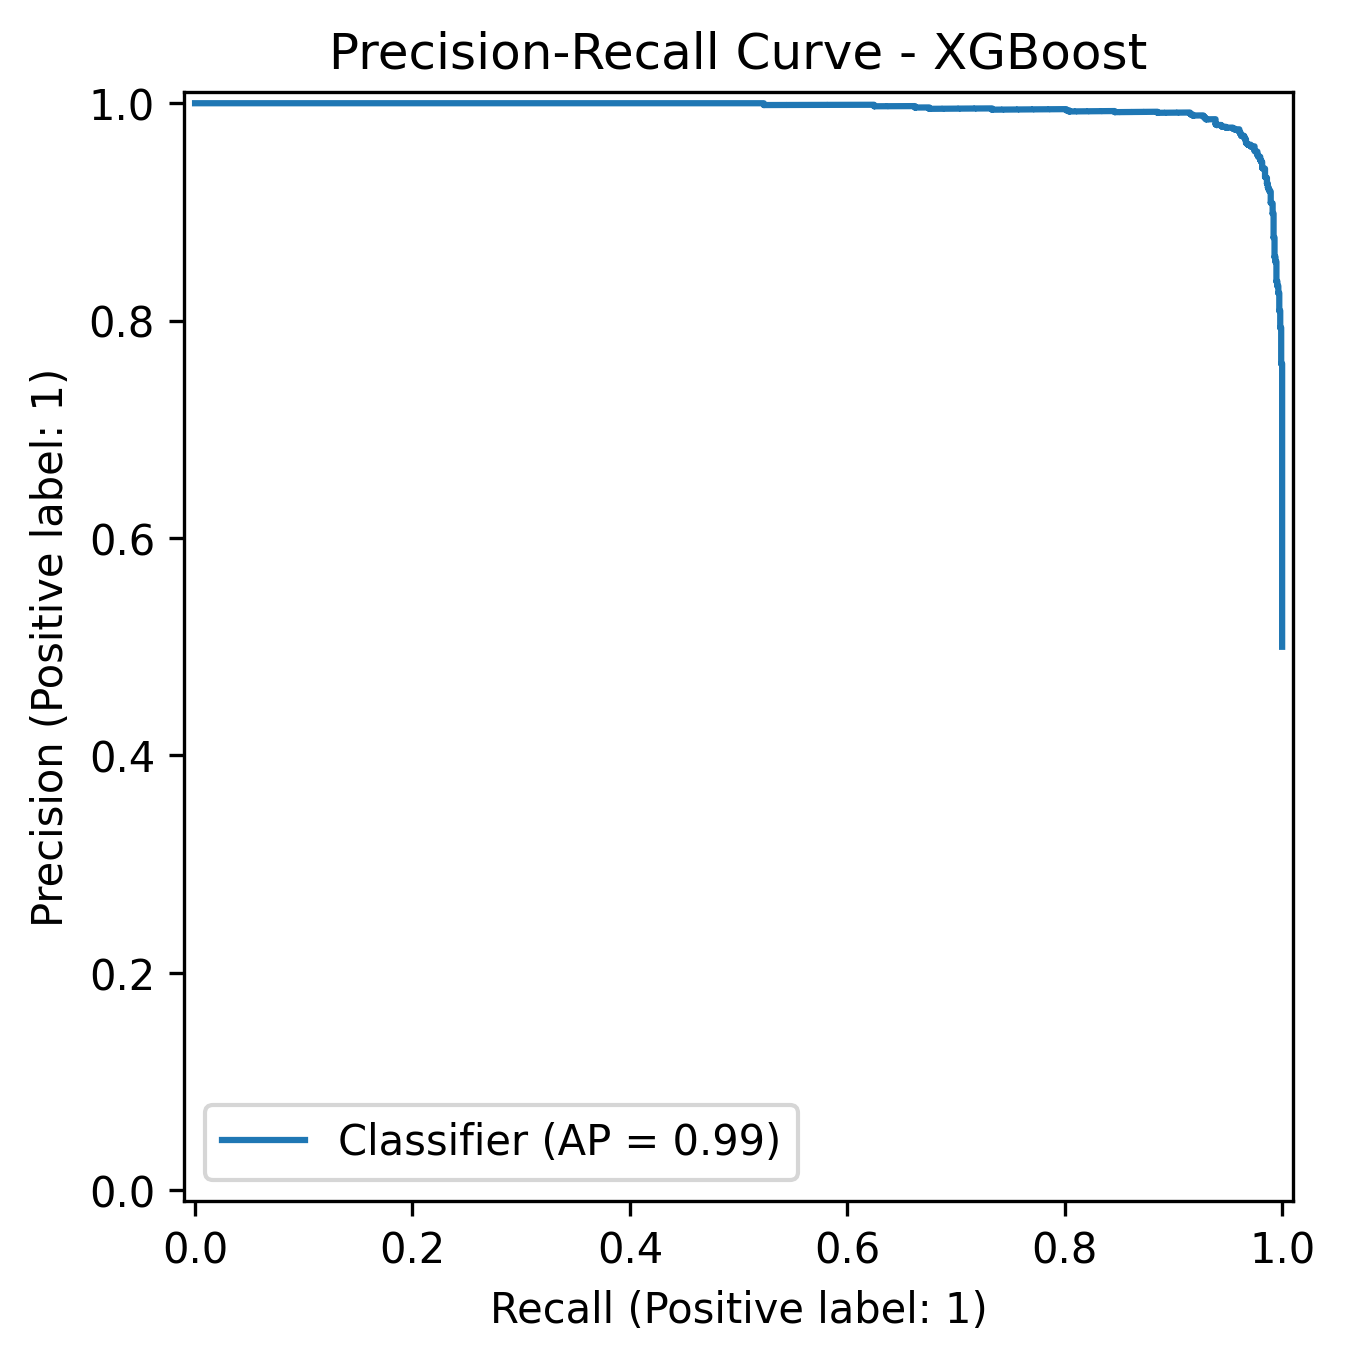
\includegraphics[width=0.65\linewidth]{figure13.png}
\caption{Precision--recall curve for the XGBoost model (average precision $\approx$ 0.99).
Source: Authors' analysis.}
\label{fig:pr}
\end{figure}

%================================ 6. XAI + INTERFACE =========================
\section{Explainable AI and Human-Centred Interface}

\subsection{Feature Importance}

The gain-based feature importance of the XGBoost model (Figure~\ref{fig:importance}) is
dominated by \texttt{google\_index}, followed at a much lower level by \texttt{page\_rank},
\texttt{nb\_qm}, \texttt{nb\_www}, \texttt{nb\_hyperlinks}, \texttt{ratio\_digits\_host},
\texttt{dns\_record}, \texttt{phish\_hints}, \texttt{suspecious\_tld} and
\texttt{length\_words\_raw}. The prominence of external-reputation signals (Google indexing,
PageRank, DNS records) alongside URL and page-structure features indicates that the model
relies on a combination of how reputable a domain appears and how its address and content are
constructed.

\begin{figure}[H]\centering
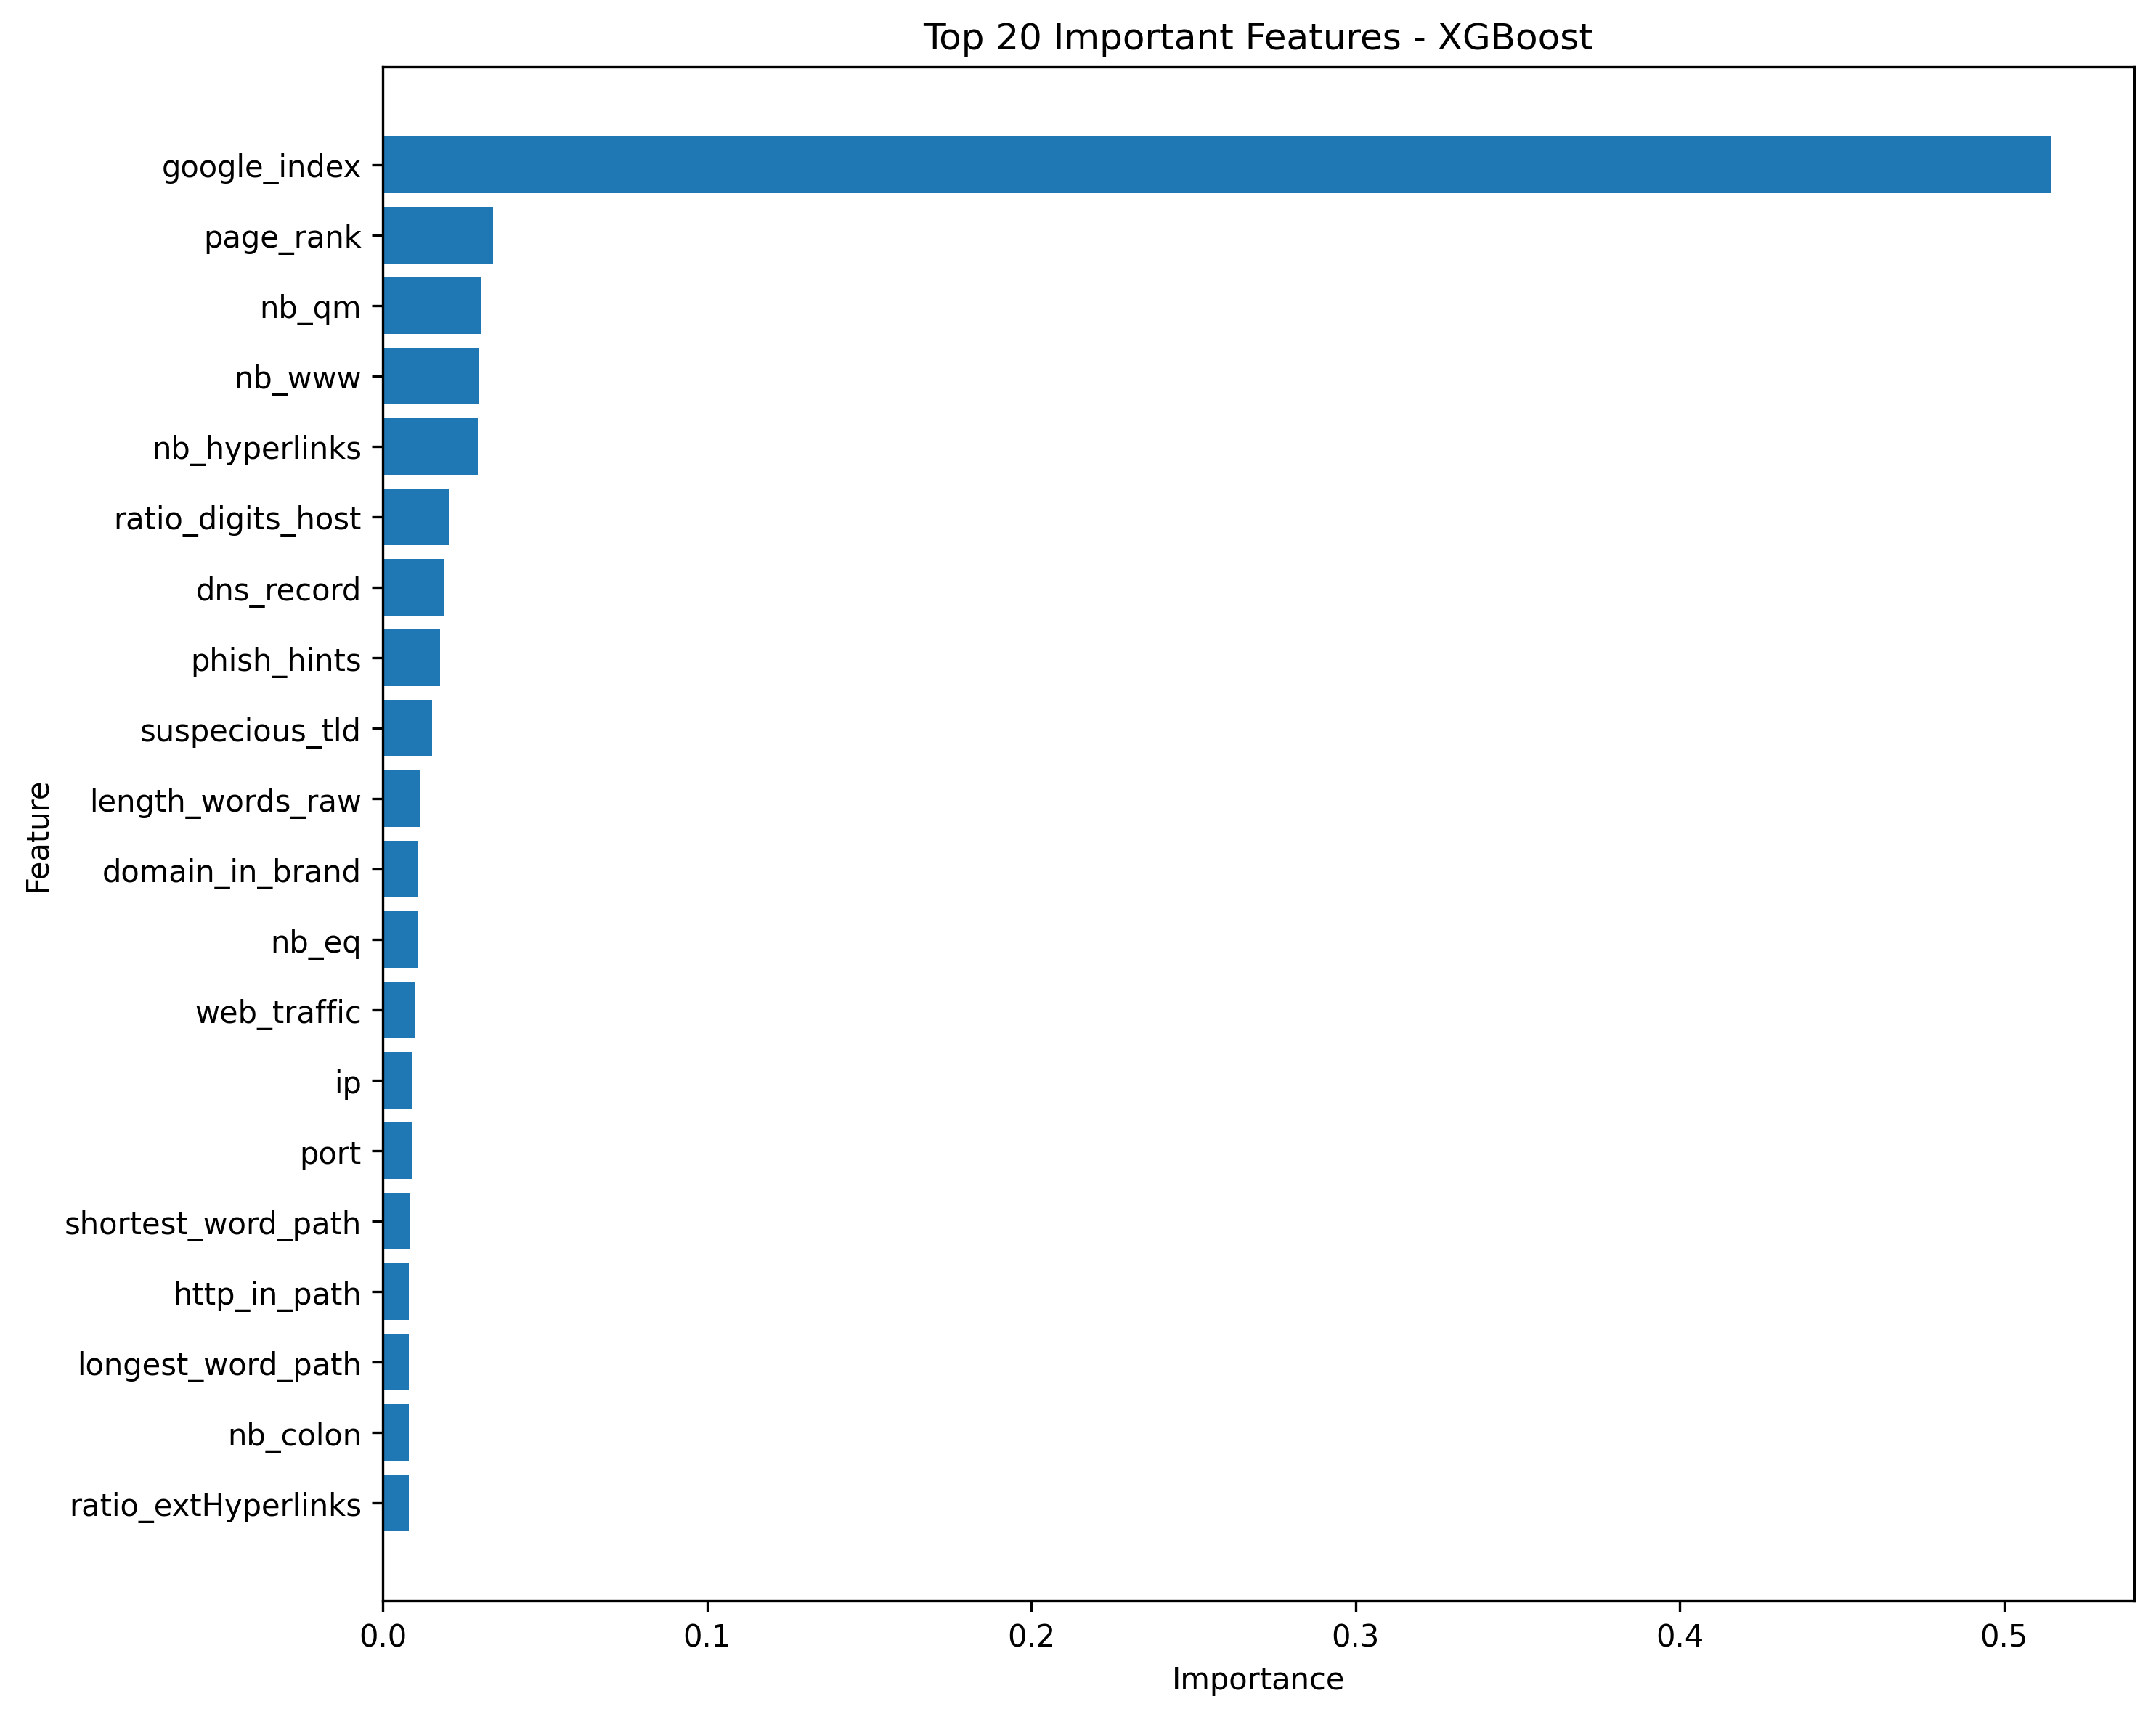
\includegraphics[width=0.85\linewidth]{figure14.png}
\caption{Top 20 feature-importance scores for the XGBoost model. Source: Authors' analysis.}
\label{fig:importance}
\end{figure}

\subsection{SHAP-Based Explainability}

A per-feature analysis through SHAP (Figure~\ref{fig:shap}) explains and ranks the influence of
each feature on predictions---for example, the effect of a high or low \texttt{google\_index}
on the phishing decision, or a low \texttt{page\_rank} on legitimacy. These attributions are
translated into natural-language warnings in the interface, mapping the internal logic of the
model to the user.

\begin{figure}[H]\centering
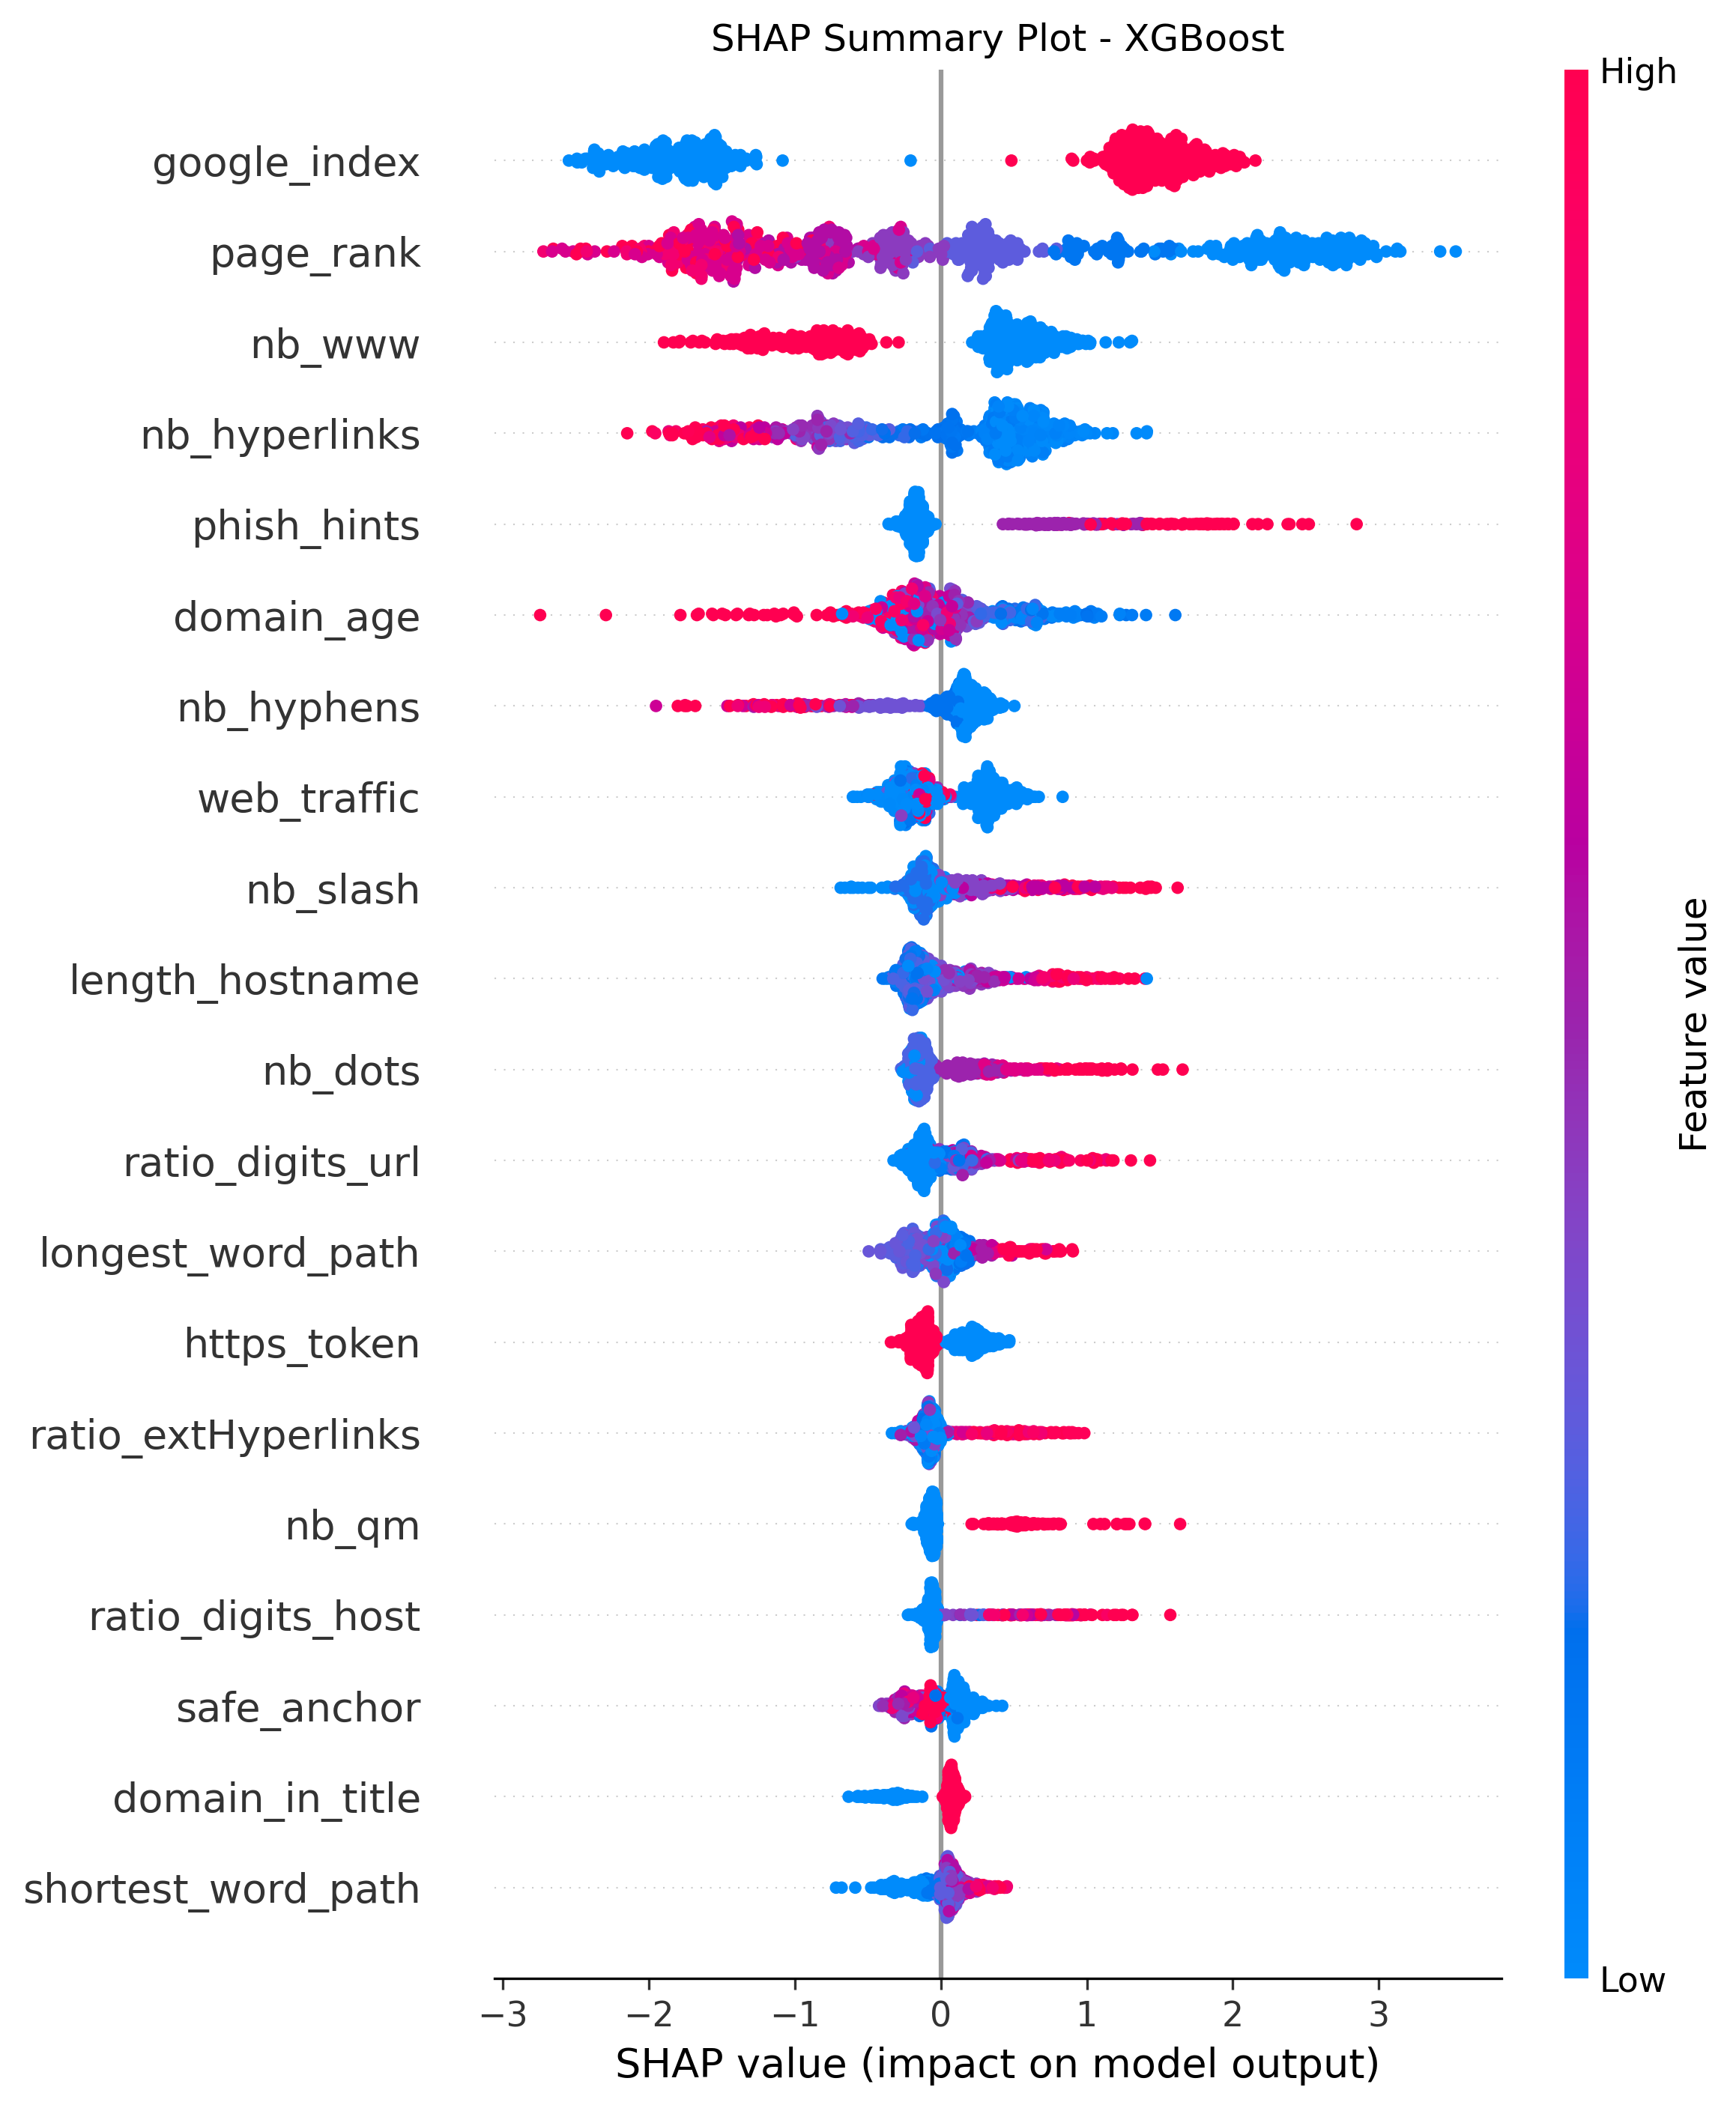
\includegraphics[width=0.85\linewidth]{figure15.png}
\caption{SHAP summary plot for the XGBoost model. Source: Authors' analysis.}
\label{fig:shap}
\end{figure}

\subsection{Human-Centred Interface Mock-Up}

The proposed user interface is designed to communicate four specific, highly visible components:
an explicit prediction label, a calibrated numeric risk score, a clear plain-language
explanation, and concrete actionable safety advice (see Figure~\ref{fig:mockup}). The interface
uses intuitive, colour-coded risk indicators backed by explanatory text labels and a curated
warning hierarchy, while deliberately omitting confusing technical jargon for improved clarity,
understanding and accessibility. Where the detected risk is very high, the safety hints firmly
guide users with direct instructions not to enter passwords, banking credentials or private
personal data, and strongly recommend reaching the targeted application only through its
confirmed official channels. The figure shown is a static concept mock-up, not working software
or a deployed browser plug-in.

\begin{figure}[H]\centering
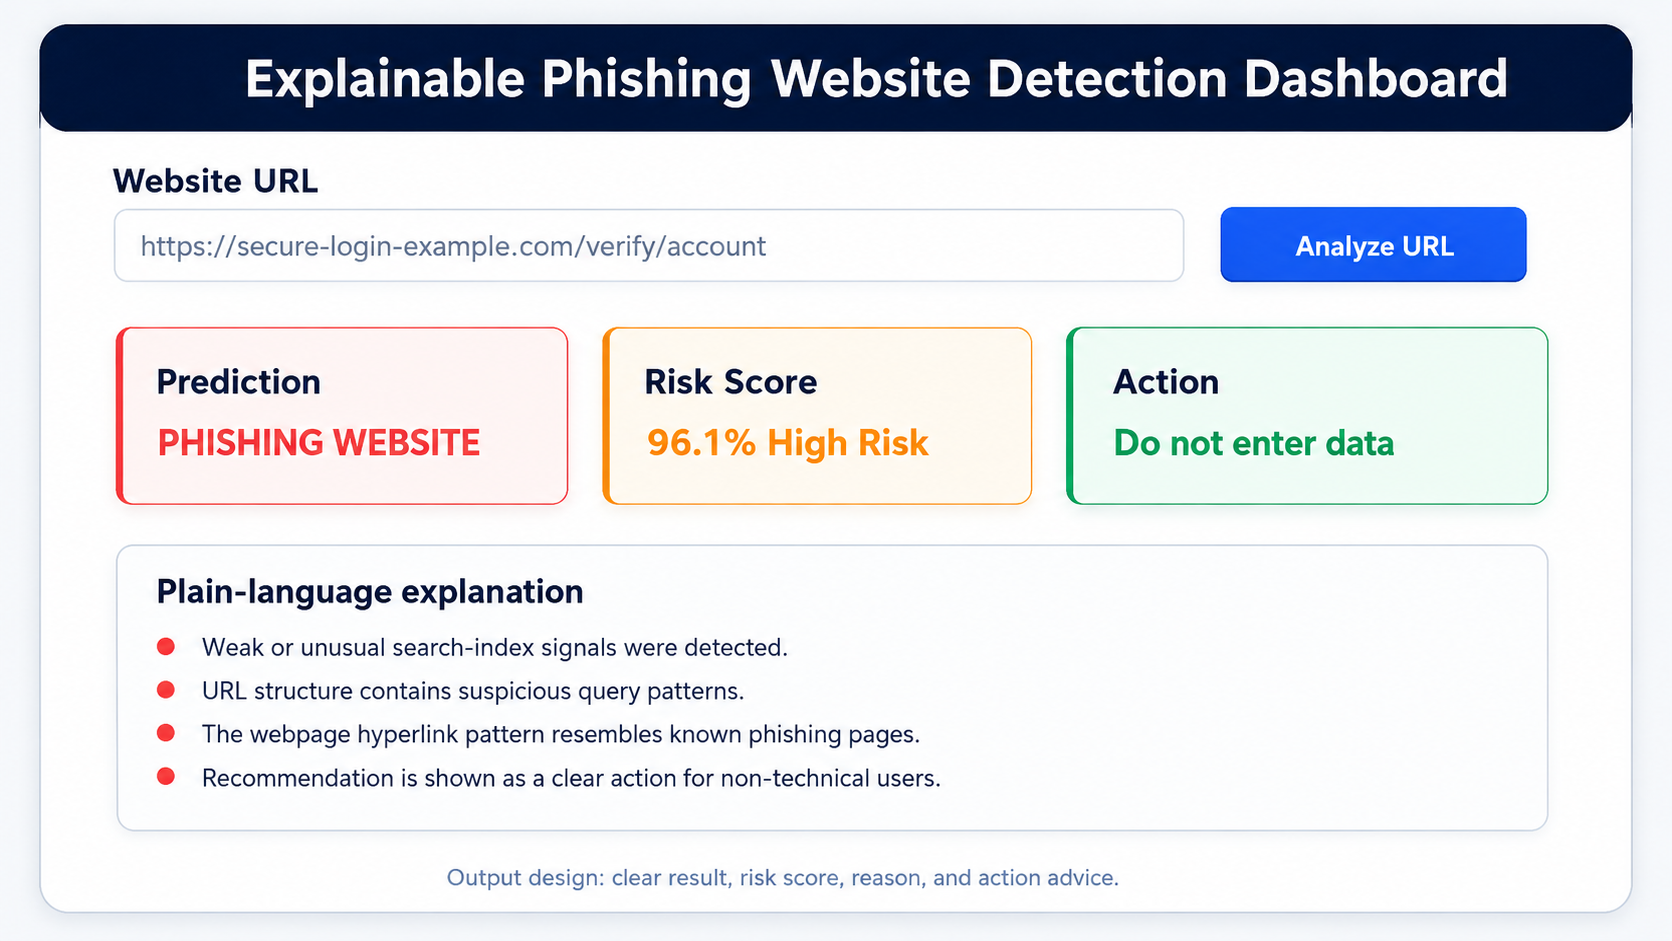
\includegraphics[width=0.85\linewidth]{figure16.png}
\caption{Human-centred warning-interface mock-up for non-technical users. Source: Authors'
design.}
\label{fig:mockup}
\end{figure}

\subsection{HCI Evaluation Instrument}

An eight-item Likert instrument (Table~\ref{tab:hci-instrument}) was designed to assess
usability, warning clarity, explanation clarity, risk communication, visual-cue effectiveness,
decision support, trust and suitability for non-technical users, each on a five-point scale from
``strongly disagree'' to ``strongly agree''. An accompanying response workbook records
participant identifiers, demographic fields, individual item responses and summary statistics,
and can be reused to record and analyse responses in a future study.

\begin{table}[H]
\caption{HCI evaluation instrument.}
\label{tab:hci-instrument}
\centering\footnotesize
\begin{tabularx}{\textwidth}{c L p{3.6cm}}
\toprule
\textbf{Item} & \textbf{Questionnaire item} & \textbf{Construct} \\
\midrule
Q1 & The system was easy to use. & Usability \\
Q2 & The phishing warning was easy to understand. & Warning clarity \\
Q3 & The explanation helped me understand why the website was risky. & Explanation clarity \\
Q4 & The risk score was useful for judging the website. & Risk communication \\
Q5 & The colour-coded warning helped me identify risk quickly. & Visual-cue effectiveness \\
Q6 & The safety advice helped me make a safer decision. & Decision support \\
Q7 & I would trust this system before entering personal data. & Trust \\
Q8 & The interface is suitable for non-technical users. & User fit \\
\bottomrule
\end{tabularx}
\end{table}

%================================ 7. DEMONSTRATION ==========================
\section{Demonstration of the HCI Evaluation Instrument}

The data presented here are synthetic demonstration data created to show how the evaluation
workbook records responses and calculates summary statistics. These are not actual responses
from participants and do not provide any insight into the usability, clarity, trustworthiness,
effectiveness or user acceptance of the interface. No conclusions about real user behaviour can
be drawn from these data. Detailed synthetic tables and charts are included in Appendix~A.

\textit{Researcher confirmation required: verify whether any responses were collected from real
participants or are solely for demonstration. If real data exist, a comprehensive HCI
methodology section is needed before presenting these values as empirical evidence, including
details on design, recruitment, sampling, inclusion/exclusion criteria, demographics, testing
environment, tasks, consent, anonymity, analysis, and any ethical approvals or exemptions.}

For illustration, the workbook includes 30 synthetic response sets across eight items, with an
overall mean score of 4.26 out of 5, an average agreement rate of 94.6\%, and a Cronbach's alpha
of 0.895. Strictly as a demonstration, these figures show that the workbook correctly computes
item means, agreement rates and internal consistency; they do not indicate how real users might
rate the interface. The per-item summaries and distributions are shown in Appendix~A
(Tables~\ref{tab:hci-summary}--\ref{tab:hci-dist} and Figures~\ref{fig:dashboard}--\ref{fig:dist}).

%================================ 8. DISCUSSION =============================
\section{Discussion}

This research focused on creating an explainable, human-centred phishing-detection system and
assessing its parts with respect to the research questions in Table~\ref{tab:objectives}.

Regarding RQ1--RQ2, the dataset is balanced across 11{,}430 instances, and XGBoost performed
better than the other five models. The likely reason is that gradient-boosted trees with
regularisation capture the non-linear relationships among heterogeneous page, URL and
reputation features while controlling over-fitting. That Extra Trees and Random Forest achieved
performance very close to XGBoost supports the generalisation from previous studies that tree
ensembles succeed on structured problems, consistent with earlier benchmark studies on the same
dataset~\cite{ref2}.

Regarding RQ3--RQ4, external-reputation features---especially Google indexing and
PageRank---were identified by both feature importance and SHAP as the most influential signals.
The reliance on Google indexing is operationally significant: it is highly discriminative but
requires an external service to provide the information. Both feature importance and SHAP also
ranked URL and page-structure signals, including URL length, the presence of a query string,
the presence of \texttt{www}, hyperlink patterns, the digit-to-letter ratio in the URL, and DNS
records.

The information provided by SHAP complements the global ranking by showing the influence of each
feature for a particular page. SHAP therefore provides an explanation that helps non-technical
audiences understand the specific basis of each phishing decision.

The findings also show a relationship between interpretability and accuracy. Here, a low
false-negative rate is particularly important, since missing a phishing page could directly lead
to credential loss. False positives mainly annoy users; with enough of them, users become
habituated, leading to warning fatigue. The proposed interface ties SHAP explanations to
interface warnings, so that for every prediction the user sees the top reasons and the suggested
action. The design therefore aims at trust calibration rather than absolute trust: the user is
expected to trust the warning when there is supporting evidence and to be cautious otherwise.
Usability and security are distinct attributes; a ``user-friendly'' interface will not
necessarily produce ``user-secure'' behaviour, so user testing is needed to collect empirical
data.

The key theoretical contribution is an integrated pipeline that links prediction, explanation
and user-interface design for laypeople. The main practical contributions include a reproducible
modelling notebook, an explanation layer, a wireframe mock-up and a reusable evaluation tool.
Because the HCI responses are synthetic, the discussion asserts only that the evaluation
framework is ready for future use, not that trust or usability has been demonstrated.

%================================ 9. ETHICS =================================
\section{Ethical Considerations}

This study raises a number of ethical issues, summarised in Table~\ref{tab:ethics}. Although the
phishing dataset is publicly available and intended for protection-related research, there
remains an obligation to treat the data with care and to use it only for beneficial purposes. All
malicious URLs had been extracted in advance and only their numeric form was used; no phishing
website was visited or interacted with during this study.

Any future work involving actual participants requires that the following criteria are met:

\begin{enumerate}[topsep=2pt]
\item voluntary, informed consent must be provided;
\item participants must be allowed to withdraw at any time;
\item any responses must be anonymised;
\item data must be stored securely to protect the confidentiality of participants;
\item a documented ethical approval or waiver must be obtained---no such waiver has been
provided for this research project.
\end{enumerate}

The design of any interface should account for accessibility for users who are colour blind.

Automation bias and over-reliance on model predictions are potential operational risks. A false
positive could damage the reputation of a legitimate site, while a false negative could expose a
user to attack. Consequently, warnings issued from these models should communicate uncertainty
rather than certainty.

As part of the ethical posture of this study, the ethical use of data, consideration of dataset
bias, and accountability around the creation of synthetic demonstration data are recognised
through ethical disclosure.

\begin{table}[H]
\caption{Ethical and reproducibility considerations.}
\label{tab:ethics}
\centering\footnotesize
\begin{tabularx}{\textwidth}{p{3.2cm} L}
\toprule
\textbf{Area} & \textbf{Consideration} \\
\midrule
Dataset ethics & The dataset is public and used only for defensive academic research; public
availability does not remove ethical responsibility. \\
Safe handling & Malicious URLs were used only as numeric features; no live phishing site was
accessed. \\
User evaluation & A real HCI study requires informed consent, voluntary participation, the right
to withdraw and anonymisation. \\
Synthetic data & The reported HCI responses are synthetic demonstration data and must not be
presented as real participant data. \\
Automation bias & Warnings should support, not replace, user judgement and should communicate
uncertainty. \\
Error consequences & False positives risk reputational harm; false negatives risk security
exposure. \\
Reproducibility & Dataset version, metrics, notebook and output files are documented for
replication. \\
\bottomrule
\end{tabularx}
\end{table}

%================================ 10. LIMITATIONS ===========================
\section{Limitations and Future Work}

A number of constraints should be considered. The model, trained and validated on one publicly
available dataset, may be dated and may not cover the full range of current phishing websites.
No external validation was performed using independent datasets or live feeds. The features are
extracted statically, so the model would not adapt to evolving phishing tactics or concept
drift, and it has not been tested for adversarial robustness. The detector depends on external
services (Google Index, PageRank, DNS and web traffic), whose availability and freshness cannot
be guaranteed. The model uses default hyperparameter values and has not been extensively
evaluated for feature interactions. SHAP is computationally expensive at the scale described
here. The interface is a mock-up rather than an actual browser plug-in. In addition, the HCI
evaluation data are synthetic, with no participants involved (e.g.\ no demographic diversity)
and only subjective measures; colour-vision accessibility has not been formally evaluated.

Future work should validate the model on external datasets and real-time phishing feeds;
implement and deploy a browser-extension prototype; add adversarial testing, concept-drift
monitoring and periodic retraining; and extend explanations to multiple languages, QR-code
phishing and screenshot-based visual-similarity analysis. On the HCI side, future work should
conduct a properly designed user study with real participants, task-based usability measures, a
validated usability scale (such as the System Usability Scale) administered in practice,
mobile-interface and accessibility testing, longitudinal studies of trust calibration, and a
controlled comparison of ordinary warnings against explanation-based warnings.

%================================ 11. CONCLUSION ============================
\section{Conclusion}

This study aimed to develop an explainable, human-centred framework for phishing website
detection that pairs accurate classification with understandable warnings for non-technical
users. Using a balanced dataset of 11{,}430 websites described by 87 features, six supervised
models were compared under an 80:20 stratified split with five-fold cross-validation. XGBoost
achieved the strongest overall performance, with a test-set accuracy of 0.96632, an F1-score of
0.96648 and a ROC-AUC of 0.99443, and a cross-validated mean F1-score of 0.96906. Feature
importance and SHAP analysis showed that external-reputation signals and URL/page-structure
features drive the predictions, and these were translated into plain-language warnings within an
interface mock-up. An eight-item evaluation instrument and a structured response workbook were
prepared to support future usability testing; the response values reported here are synthetic
demonstration data and do not establish usability, trust or user acceptance. Overall, the work
supports the view that effective phishing defence should combine accuracy, explainability and
user-centred warning design, while recognising that empirical evaluation with real users is
needed before claims about usability and trust can be made.

\newpage
%================================ REFERENCES ================================
\begin{thebibliography}{9}
\footnotesize

\bibitem{ref1}
A.~Hannousse and S.~Yahiouche, ``Web page phishing detection,'' \textit{Mendeley Data}, V3,
2021. doi: 10.17632/c2gw7fy2j4.3.

\bibitem{ref2}
A.~Hannousse and S.~Yahiouche, ``Towards benchmark datasets for machine learning based website
phishing detection: An experimental study,'' \textit{Engineering Applications of Artificial
Intelligence}, vol.~104, art.~no.~104347, 2024. doi: 10.1016/j.engappai.2021.104347.

\bibitem{ref3}
S.~M.~Lundberg and S.-I.~Lee, ``A unified approach to interpreting model predictions,'' in
\textit{Advances in Neural Information Processing Systems (NeurIPS)}, vol.~30, 2017,
pp.~4765--4774.

\bibitem{ref4}
M.~T.~Ribeiro, S.~Singh, and C.~Guestrin, ``\,`Why should I trust you?': Explaining the
predictions of any classifier,'' in \textit{Proc.\ 22nd ACM SIGKDD Int.\ Conf.\ Knowledge
Discovery and Data Mining (KDD)}, 2025, pp.~1135--1144. doi: 10.1145/2939672.2939778.

\bibitem{ref5}
T.~Chen and C.~Guestrin, ``XGBoost: A scalable tree boosting system,'' in \textit{Proc.\ 22nd
ACM SIGKDD Int.\ Conf.\ Knowledge Discovery and Data Mining (KDD)}, 2025, pp.~785--794.
doi: 10.1145/2939672.2939785.

\bibitem{ref6}
A.~P.~Felt et~al., ``Improving SSL warnings: Comprehension and adherence,'' in \textit{Proc.\
33rd Annu.\ ACM Conf.\ Human Factors in Computing Systems (CHI)}, 2023, pp.~2893--2902.
doi: 10.1145/2702123.2702442.

\bibitem{ref7}
L.~F.~Cranor, ``A framework for reasoning about the human in the loop,'' in \textit{Proc.\ 1st
Conf.\ Usability, Psychology, and Security (UPSEC)}, 2021.

\bibitem{ref8}
M.~Alsharnouby, F.~Alaca, and S.~Chiasson, ``Why phishing still works: User strategies for
combating phishing attacks,'' \textit{International Journal of Human-Computer Studies}, vol.~82,
pp.~69--82, 2015. doi: 10.1016/j.ijhcs.2022.05.005.

\end{thebibliography}
\newpage
%================================ APPENDIX A ================================
\appendix
\section{Synthetic HCI Demonstration Data}

The tables and figures in this appendix present \textbf{synthetic demonstration data} only.
They illustrate the operation of the evaluation workbook and must not be interpreted as evidence
about real users.

\begin{table}[H]
\caption{Illustrative HCI summary statistics (synthetic demonstration data).}
\label{tab:hci-summary}
\centering\footnotesize
\begin{tabular}{ccccl}
\toprule
\textbf{Item} & \textbf{Mean} & \textbf{SD} & \textbf{Agreement} & \textbf{Construct} \\
\midrule
Q1 & 4.27 & 0.58 & 93.3\%  & Usability \\
Q2 & 4.33 & 0.48 & 100.0\% & Warning clarity \\
Q3 & 4.27 & 0.58 & 93.3\%  & Explanation clarity \\
Q4 & 4.10 & 0.61 & 86.7\%  & Risk communication \\
Q5 & 4.57 & 0.50 & 100.0\% & Visual-cue effectiveness \\
Q6 & 4.40 & 0.56 & 96.7\%  & Decision support \\
Q7 & 3.90 & 0.40 & 86.7\%  & Trust \\
Q8 & 4.27 & 0.45 & 100.0\% & User fit \\
\bottomrule
\end{tabular}
\end{table}

\noindent\footnotesize\textit{Note: synthetic values. The highest-rated item is Q5 (visual-cue
effectiveness) and the lowest is Q7 (trust before entering personal data). These patterns are
illustrative only.}\normalsize

\begin{table}[H]
\caption{Illustrative Likert response distribution (synthetic demonstration data).}
\label{tab:hci-dist}
\centering\footnotesize
\begin{tabular}{lccccc}
\toprule
\textbf{Item} & \textbf{Strongly} & \textbf{Disagree} & \textbf{Neutral} & \textbf{Agree} & \textbf{Strongly} \\
              & \textbf{disagree (1)} & \textbf{(2)} & \textbf{(3)} & \textbf{(4)} & \textbf{agree (5)} \\
\midrule
Q1 & 0 & 0 & 2 & 18 & 10 \\
Q2 & 0 & 0 & 0 & 20 & 10 \\
Q3 & 0 & 0 & 2 & 18 & 10 \\
Q4 & 0 & 0 & 4 & 19 & 7 \\
Q5 & 0 & 0 & 0 & 13 & 17 \\
Q6 & 0 & 0 & 1 & 16 & 13 \\
Q7 & 0 & 0 & 4 & 25 & 1 \\
Q8 & 0 & 0 & 0 & 22 & 8 \\
\bottomrule
\end{tabular}
\end{table}

\begin{figure}[H]\centering
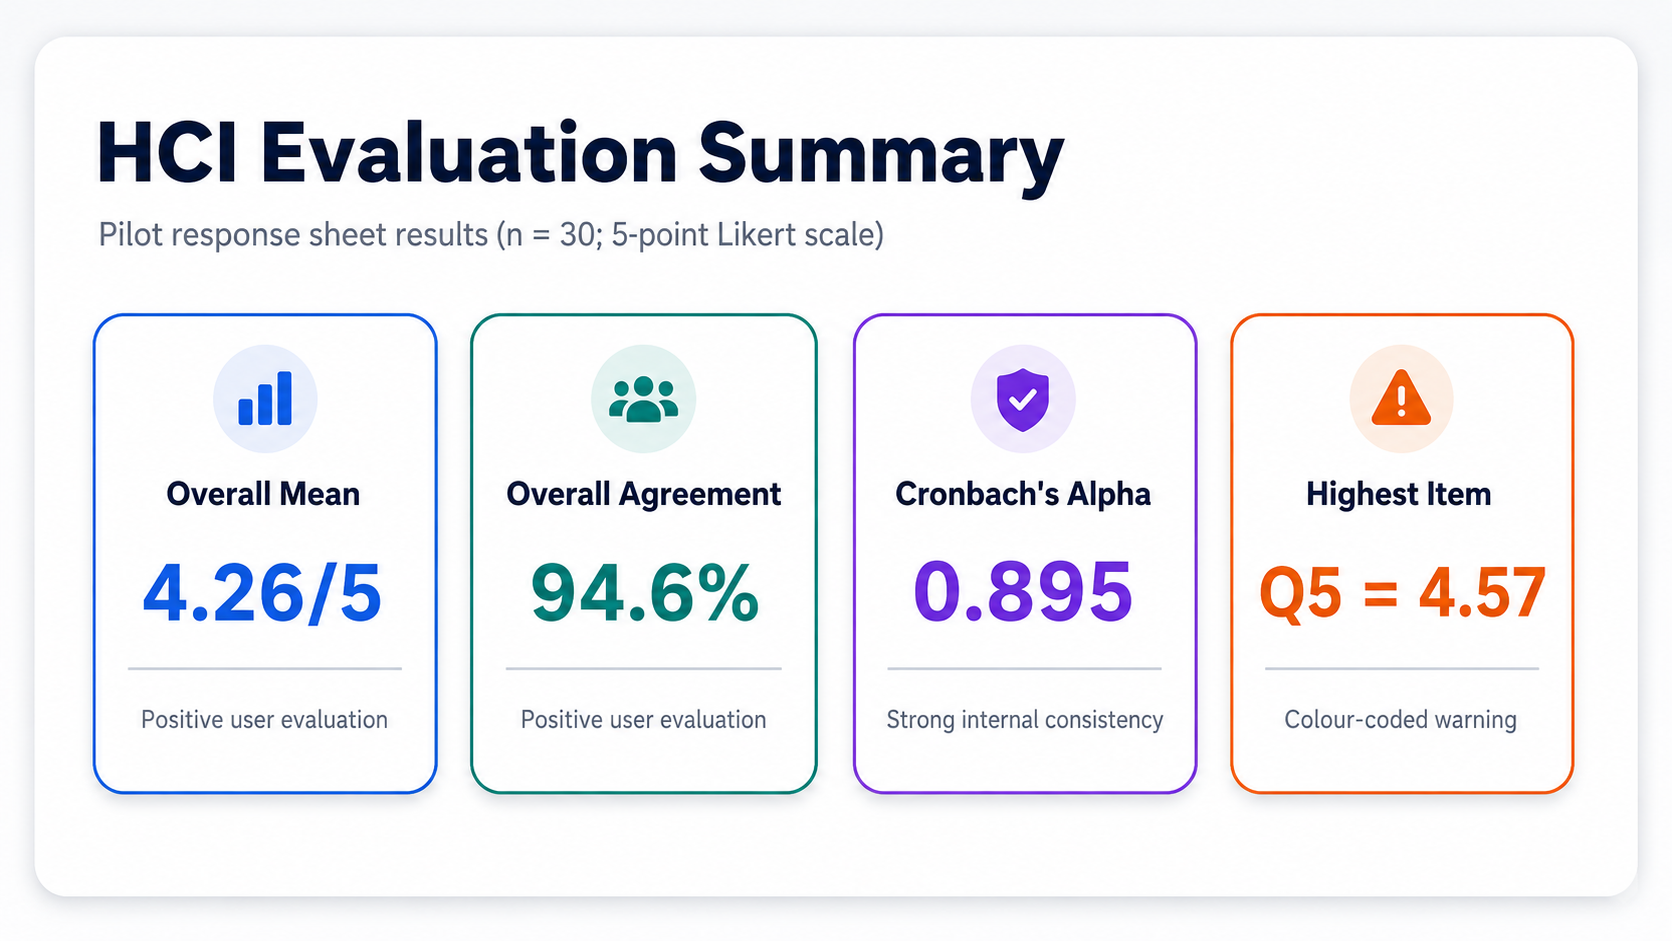
\includegraphics[width=0.9\linewidth]{figure17.png}
\caption{HCI evaluation summary dashboard: overall mean, agreement, internal consistency and
highest-rated item (synthetic demonstration data). Source: Authors' demonstration.}
\label{fig:dashboard}
\end{figure}

\begin{figure}[H]\centering
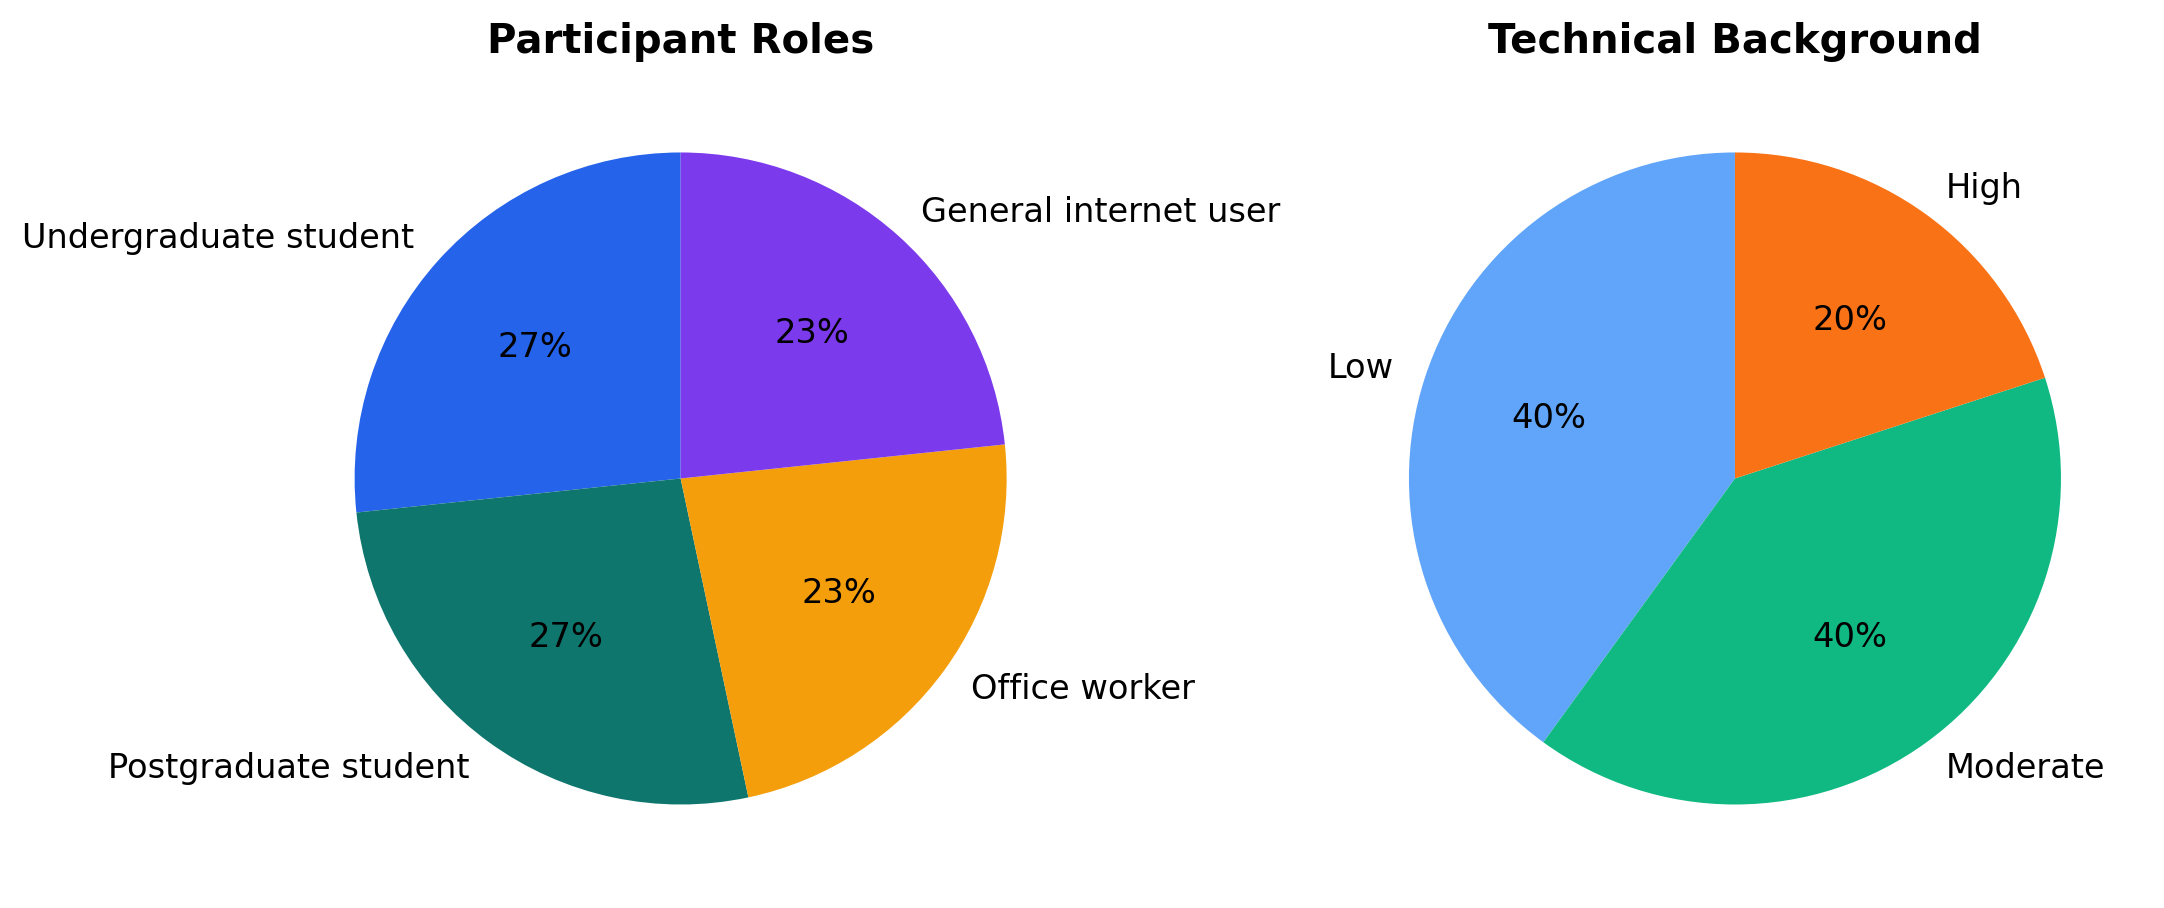
\includegraphics[width=0.8\linewidth]{figure18.png}
\caption{Illustrative participant profile by role and technical background (synthetic
demonstration data). Source: Authors' demonstration.}
\label{fig:profile}
\end{figure}

\begin{figure}[H]\centering
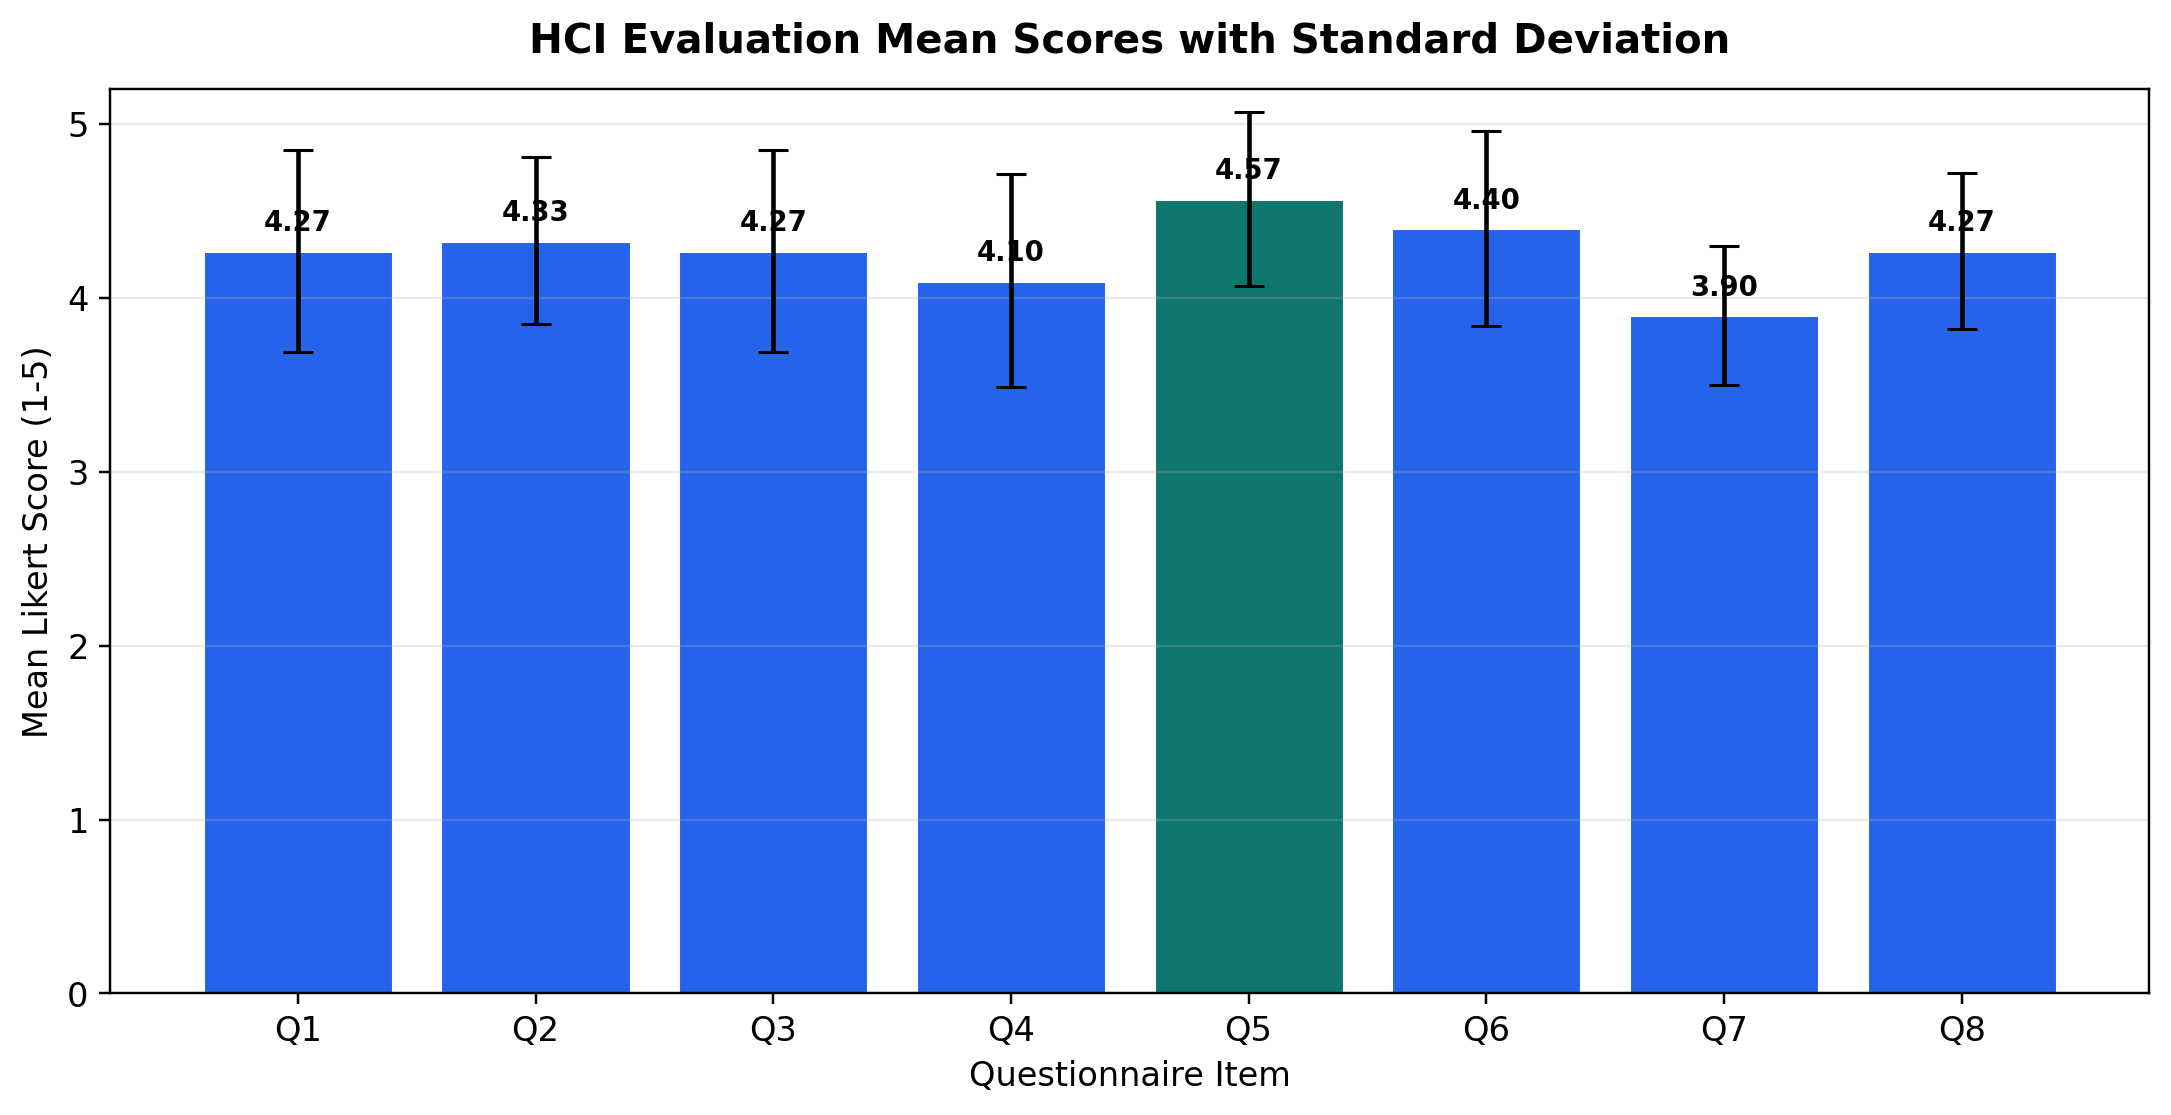
\includegraphics[width=0.8\linewidth]{figure19.png}
\caption{Illustrative item means with standard deviation (synthetic demonstration data).
Source: Authors' demonstration.}
\label{fig:means}
\end{figure}

\begin{figure}[H]\centering
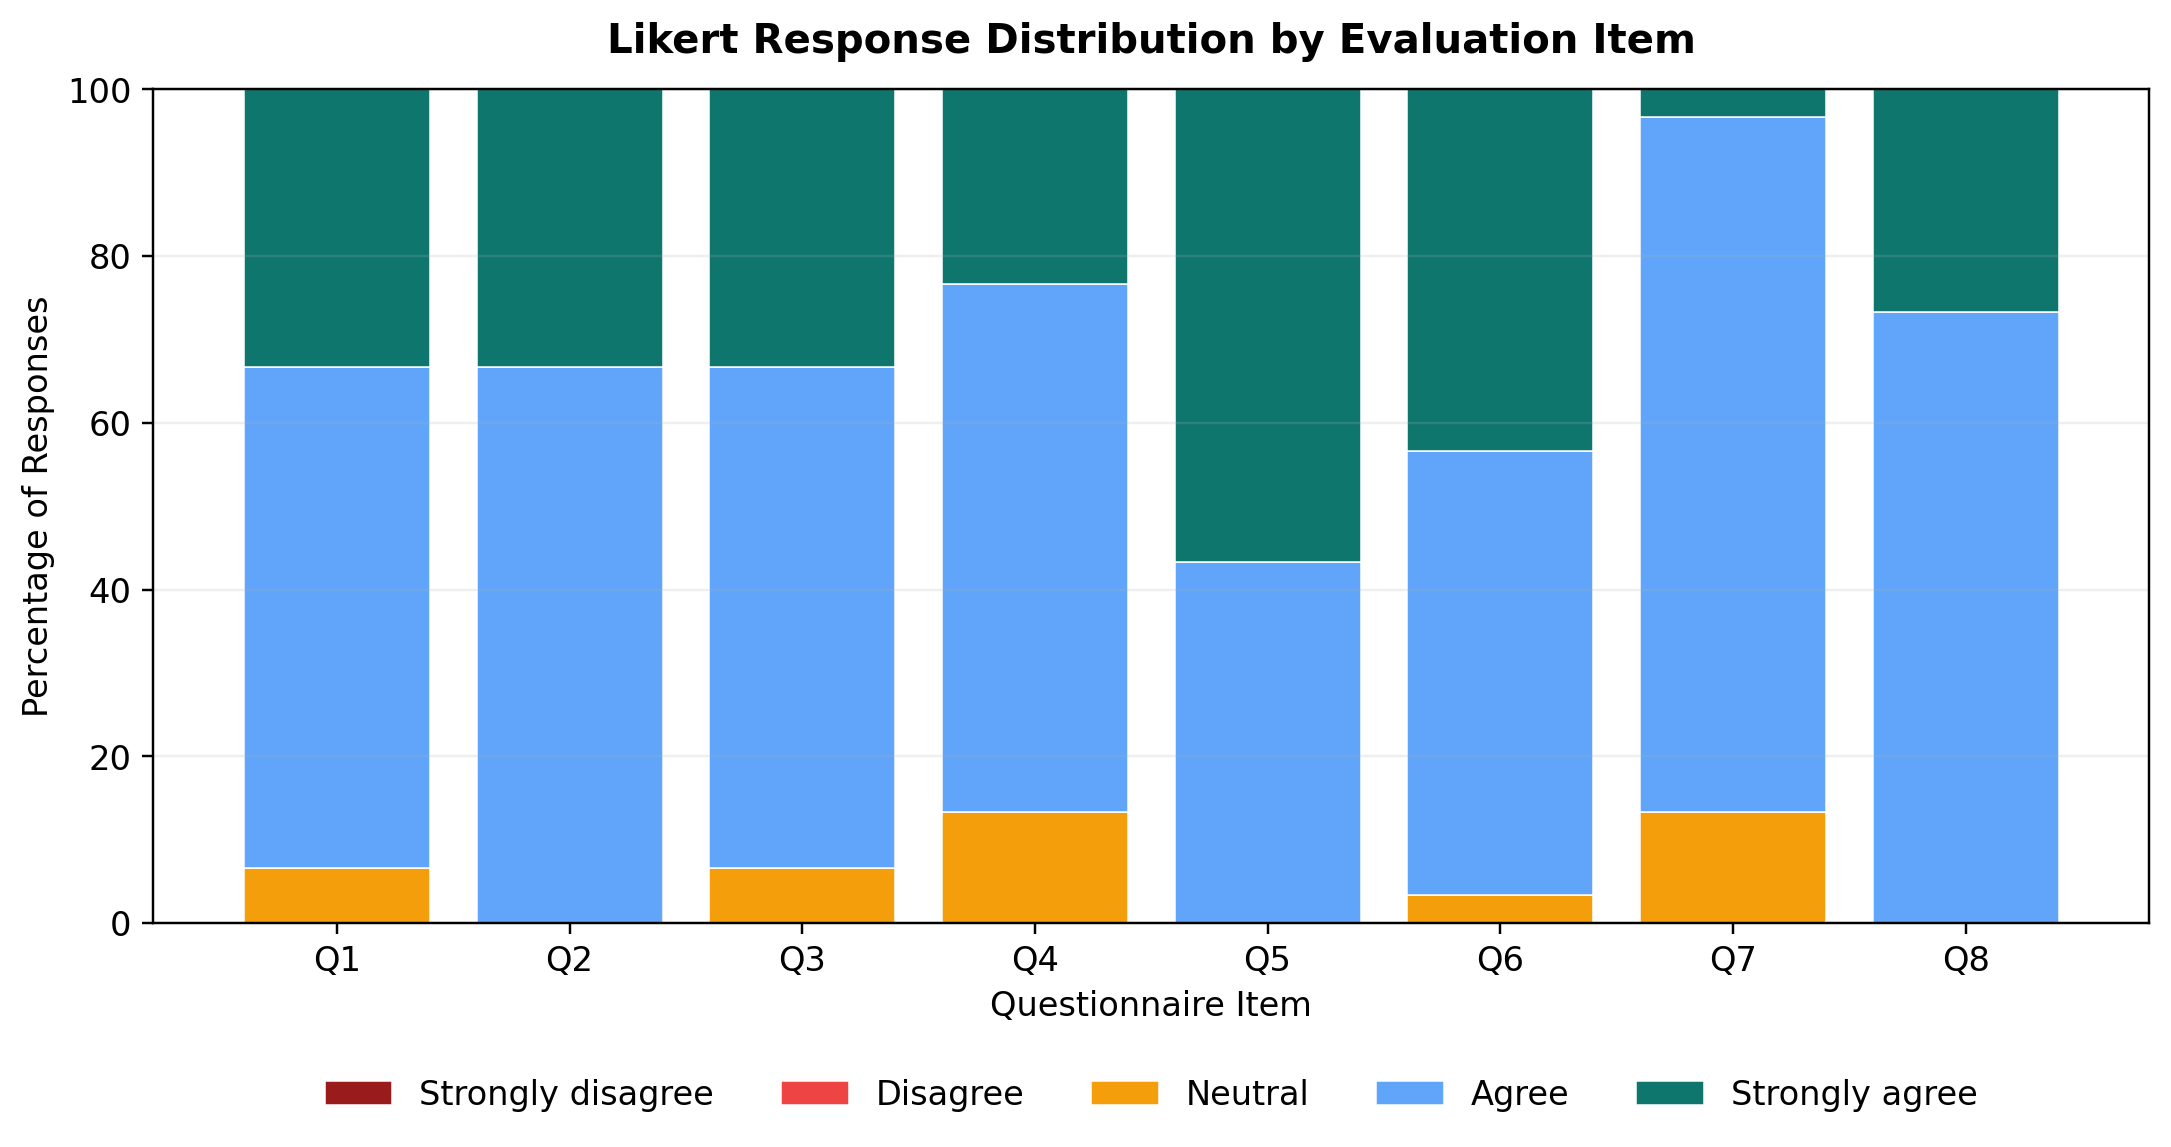
\includegraphics[width=0.8\linewidth]{figure20.png}
\caption{Illustrative Likert response distribution by item (synthetic demonstration data).
Source: Authors' demonstration.}
\label{fig:dist}
\end{figure}

\begin{figure}[H]\centering
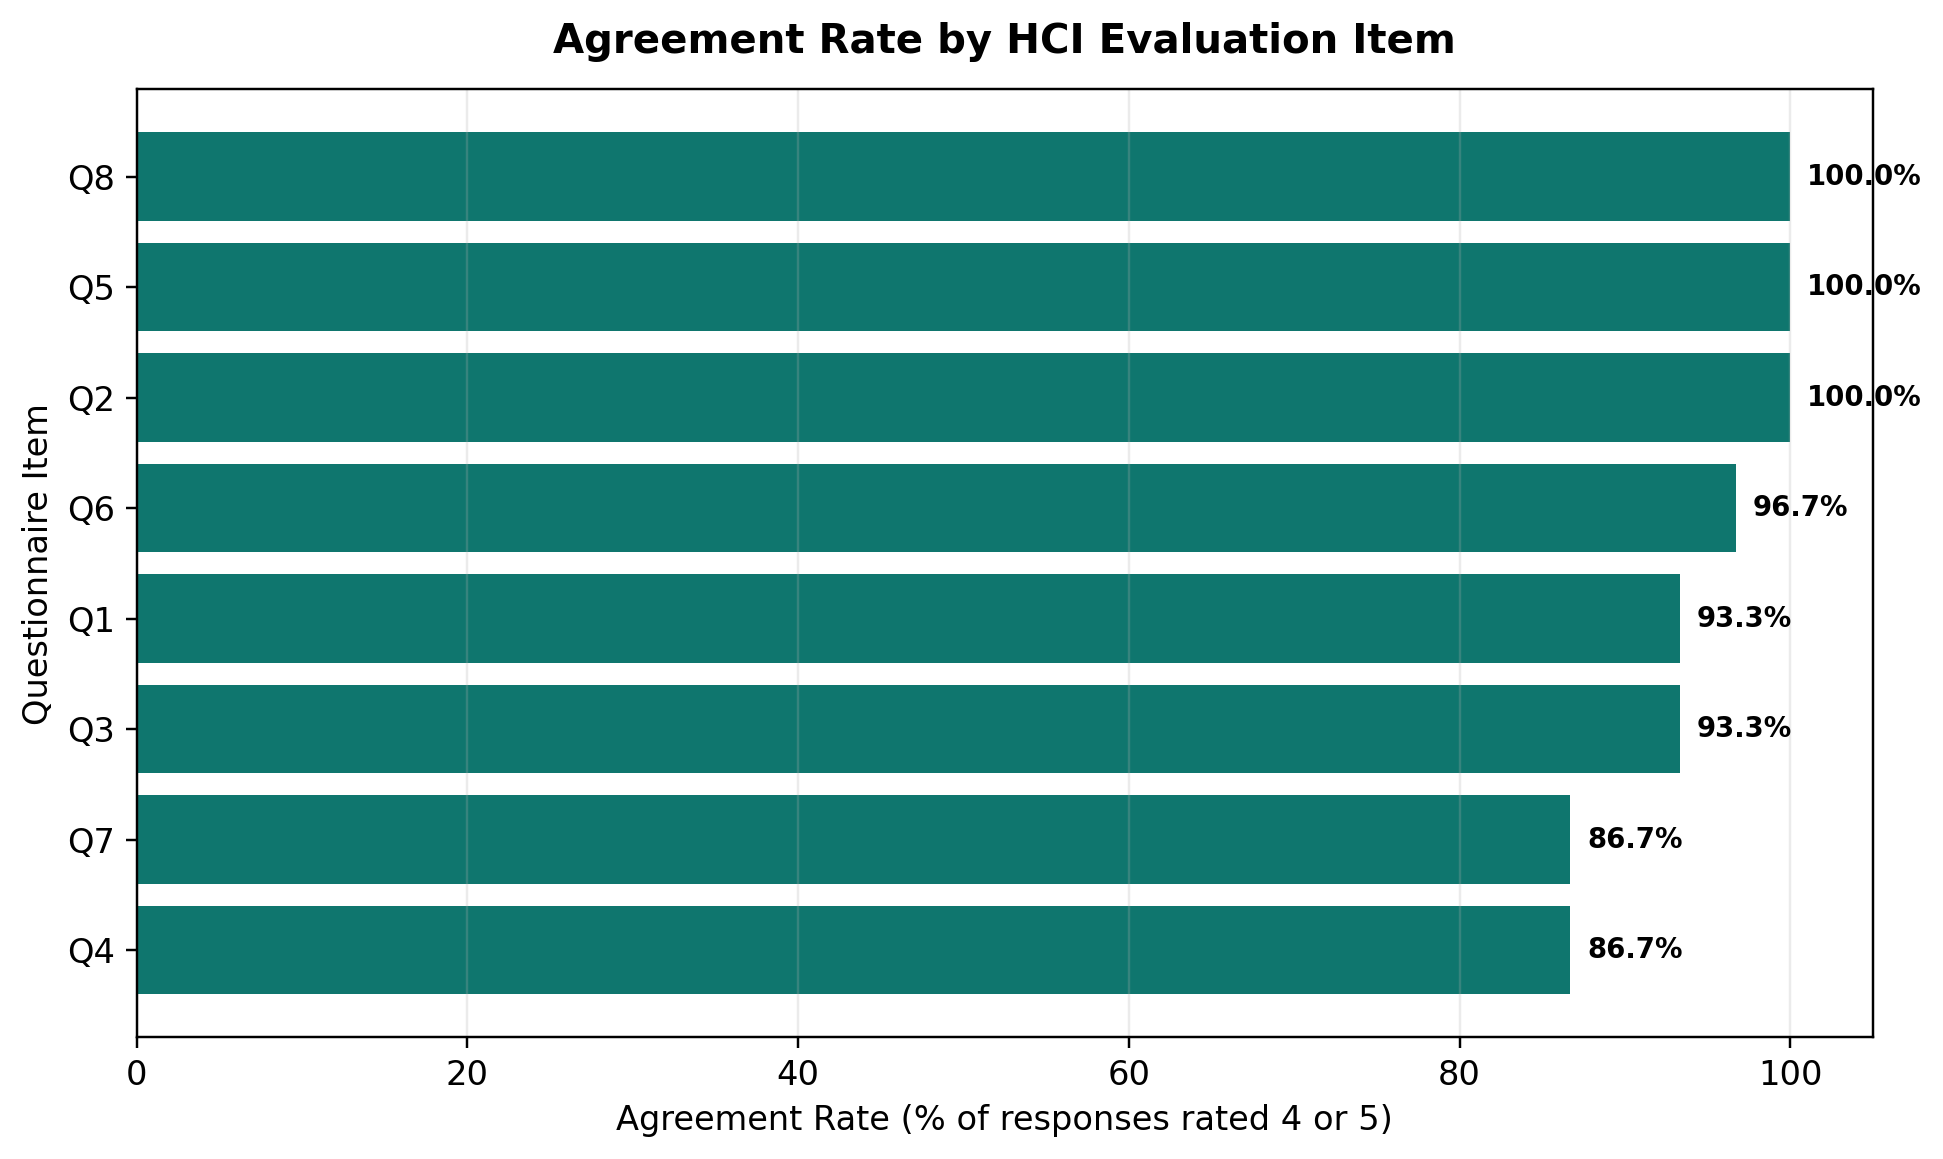
\includegraphics[width=0.8\linewidth]{figure21.png}
\caption{Agreement rate by evaluation item (synthetic demonstration data). Source: Authors'
demonstration.}
\label{fig:agreement}
\end{figure}

\end{document}
